\section{Friction model}

The current effort measured by the ESCON controller is \textcolor{green}{proportional} to the sum of the force required to overcome the nonlinearities of the EndoWrist and the external forces applied to the end-effector. One of the main nonlinearities is the friction. For the system to be transparent, the force required to overcome friction should not be fed back as this force would not be felt if the teleoperator was holding the tool directly. In order to isolate the external forces, a friction model is required. The model built is based on the one derived in \cite{force_reflection} that describe the friction in a motor. However in the model it was decided to consider the motor and the EndoWrist as one element as no dynamic model for the motor alone is derived. Thus, the model estimates the sum of the friction in the EndoWrist and in the motor.

\subsection{Model}
The total friction acting on the actuator can be written as:
\vspace{9pt}
\begin{equation}
\tau_f = \tau_v + \tau_c + \tau_s
\label{eq:total_friction}
\end{equation} 

with:\\
\hspace*{8mm} $\tau_v$ viscous friction\\
\hspace*{8mm} $\tau_c$ coulomb friction\\
\hspace*{8mm} $\tau_s$ static friction    


The viscous friction is proportional to the opposite of the velocity:
\begin{equation}
\tau_v = F_\mu \cdot \omega
\label{eq:viscous_friction}
\end{equation}
with:\\
\hspace*{8mm}$\omega$ the angular velocity\\
\hspace*{8mm}$F_\mu$ a negative coefficient\\

The coefficient $F_\mu$ can be computed from the measurements made on the setup by plotting the effort depending on the velocity.

The stiction or static friction is the amount of effort required for the object to start moving when its velocity is zero. As such it can be described as:
\vspace{9pt}
\begin{equation} 
\tau_s =  \begin{cases} K_s, & \mbox{if } \omega = 0 \\ 0, & \mbox{else} \end{cases}
\label{eq:static_friction}
\end{equation}
with:\\
\hspace*{8mm}$\omega$ the angular velocity\\
\hspace*{8mm}$K_s$ a constant\\

%The constant $K_s$ can be measured by increasing the current supplied to the motor until it starts moving. 
The coulomb friction occurs as a constant force opposing the movement:

\begin{equation}
\tau_c = sign(\omega)\cdot K_c
\label{eq:coulomb_friction}
\end{equation}
with:\\
\hspace*{8mm}$\omega$ the angular velocity\\
\hspace*{8mm}$K_c$ a constant determined experimentally\\
\hspace*{8mm}the $sign$ function is defined as $sign(\omega) = \begin{cases} 1, & \mbox{if } \omega > 0 \\ 0, & \mbox{if } \omega == 0 \\ -1, & \mbox{if } \omega < 0\end{cases}$\\

%The constant $K_c$ can be measured by setting the motor in motion and decreasing the current until the motor stops moving.
From \eqref{eq:viscous_friction} to \eqref{eq:coulomb_friction}, the total friction given by \eqref{eq:total_friction} can be plotted as:

\begin{figure}[h]
\centering
	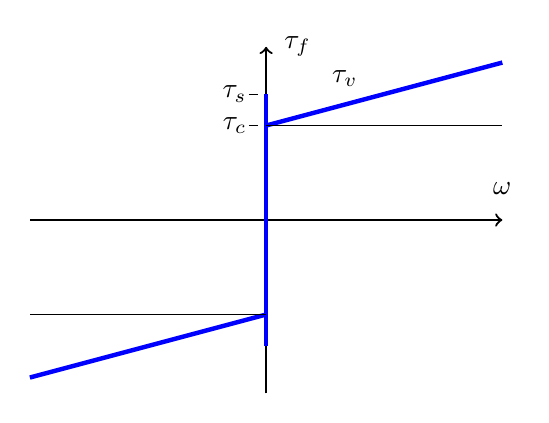
\begin{tikzpicture}
	%axes
	\draw [->,thick] (-3,0) -- (3,0);
	\draw [->,thick] (0,-2.2) -- (0,2.2);
	%friction model
	\draw [ultra thick, color=blue] (0,-1.6) -- (0,1.6);
	\draw [ultra thick, color=blue] (0,1.2) -- (3,2);
	\draw [ultra thick, color=blue] (0,-1.2) -- (-3,-2);
	\draw (0,1.2) -- (3,1.2);
	\draw (0,-1.2) -- (-3,-1.2);
	%name of axis and variables
	\node at (-0.4,1.6) {$\tau_s$};
	\draw (-0.22,1.6) -- (-0.1,1.6);
	\node at (-0.4,1.2) {$\tau_c$};
	\draw (-0.22,1.2) -- (-0.1,1.2);
	\node at (1,1.8) {$\tau_v$};


	\node at (3,0.4) {$\omega$};
	\node at (0.4,2.2) {$\tau_f$};

	\end{tikzpicture}
\caption{friction model}
\end{figure}

\subsection{Measurements}

For the model to be complete, each type of friction requries a value to be measured. These measurements need to be made for each joint as the nonlinearities in the EndoWrist varies greatly depending on the joints.

\subsection*{Test equipment:}

\begin{itemize}
	\item Endowrist model 420093 (AAU number: \#4).
	\item Maxon 110160 motor with attached Maxon gearhead 110356 and Maxon encoder 201937.
	\item sbRIO board.
\end{itemize}

\subsection*{Procedure:}
The viscous friction coefficient $F$ can be calculated by measuring the current for different speeds. From these values, an affine function can be computed, the slope of which will be the coefficient.
The constant $K_c$ for the Coulomb friction can be measured by setting the motor in motion and decreasing the current until it stops moving. The value of the current at that time is the value of $K_c$.
The constant $K_s$ for the static friction is measured by increasing the current sent to the motor until it starts moving. The value of the current at that time is the value of $K_s$.

This procedure is repeated for each motors.

\subsection*{Measuring data:}
\begin{figure}[H]
	\centering
	% This file was created by matlab2tikz.
%
%The latest updates can be retrieved from
%  http://www.mathworks.com/matlabcentral/fileexchange/22022-matlab2tikz-matlab2tikz
%where you can also make suggestions and rate matlab2tikz.
%
\definecolor{mycolor1}{rgb}{0.00000,0.44700,0.74100}%
%
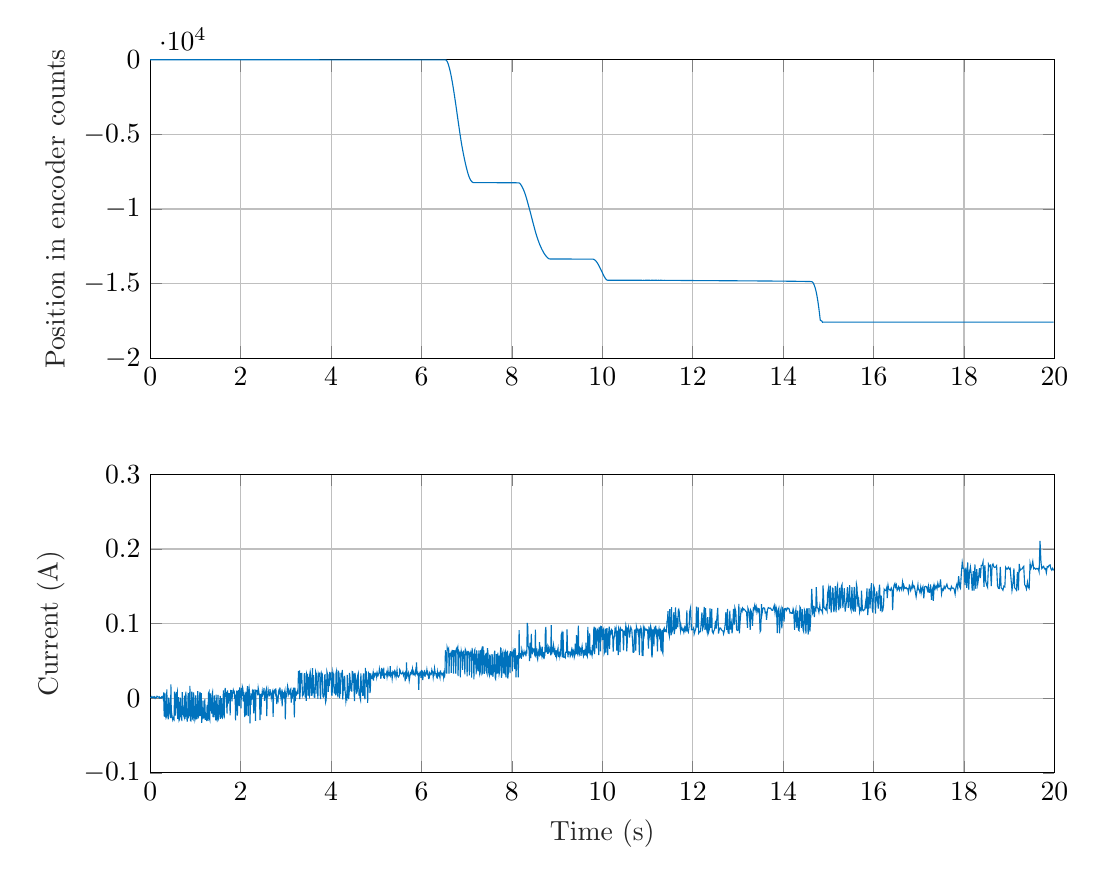
\begin{tikzpicture}

\begin{axis}[%
width=4.521in,
height=1.493in,
at={(0.758in,2.554in)},
scale only axis,
xmin=0,
xmax=20,
ymin=-20000,
ymax=0,
ylabel style={font=\color{white!15!black}},
ylabel={Position in encoder counts},
axis background/.style={fill=white},
xmajorgrids,
ymajorgrids
]
\addplot [color=mycolor1, forget plot]
  table[row sep=crcr]{%
0	0\\
0.02725744	0\\
0.03728676	0\\
0.04958916	0\\
0.05725431	0\\
0.06728411	0\\
0.07726097	0\\
0.08731127	0\\
0.09955502	0\\
0.10726881	0\\
0.11729431	0\\
0.12728214	0\\
0.13732958	0\\
0.14959764	0\\
0.15727186	0\\
0.16730928	0\\
0.17729568	0\\
0.18732214	0\\
0.19960022	0\\
0.20727921	0\\
0.21731997	0\\
0.22730112	0\\
0.23733616	0\\
0.24961329	0\\
0.2572937	0\\
0.26732731	0\\
0.27731371	0\\
0.28735065	0\\
0.29959202	0\\
0.30730677	0\\
0.31734419	0\\
0.32732582	0\\
0.33737564	0\\
0.3496027	0\\
0.35731268	0\\
0.36734486	0\\
0.37733603	0\\
0.38736629	0\\
0.39964342	0\\
0.40732479	0\\
0.41736126	0\\
0.4273448	0\\
0.43737841	0\\
0.44964027	0\\
0.45734119	0\\
0.46736956	0\\
0.4773531	0\\
0.48740482	0\\
0.49970484	0\\
0.50735998	0\\
0.51738071	0\\
0.52736855	0\\
0.5374155	0\\
0.54968071	0\\
0.55737114	0\\
0.56739426	0\\
0.57738066	0\\
0.58742189	0\\
0.59969187	0\\
0.60736847	0\\
0.61739826	0\\
0.62739182	0\\
0.63743448	0\\
0.6498127	0\\
0.6573782	0\\
0.66741371	0\\
0.67740965	0\\
0.68744802	0\\
0.6997385	0\\
0.70739174	0\\
0.71743107	0\\
0.72741556	0\\
0.73748016	0\\
0.74978542	0\\
0.75740576	0\\
0.76743746	0\\
0.77744055	0\\
0.7874999	0\\
0.79983044	0\\
0.80741215	0\\
0.8174634	0\\
0.82744026	0\\
0.83748913	0\\
0.84976864	0\\
0.85742188	0\\
0.86746073	0\\
0.87744856	0\\
0.88750172	0\\
0.89989138	0\\
0.90744638	0\\
0.91746902	0\\
0.92746115	0\\
0.93750048	0\\
0.94980145	0\\
0.9574604	0\\
0.96748018	0\\
0.97746754	0\\
0.98752213	0\\
0.99978924	0\\
1.00746536	0\\
1.01749325	0\\
1.02748632	0\\
1.0375247	0\\
1.04981041	0\\
1.05747461	0\\
1.06752253	0\\
1.07748842	0\\
1.08753395	0\\
1.09983158	0\\
1.10748911	0\\
1.11750937	0\\
1.12750673	0\\
1.137537	0\\
1.14986134	0\\
1.15749264	0\\
1.16752291	0\\
1.17751884	0\\
1.18754292	0\\
1.19987154	0\\
1.20751095	0\\
1.21753025	0\\
1.22752142	0\\
1.23756742	0\\
1.24991846	0\\
1.25751448	0\\
1.26753855	0\\
1.27752399	0\\
1.28757811	0\\
1.29983902	0\\
1.3075285	0\\
1.3175602	0\\
1.32754993	0\\
1.33758974	0\\
1.34985828	0\\
1.35754061	0\\
1.36755753	0\\
1.37754869	0\\
1.38757658	0\\
1.39988708	0\\
1.40755272	0\\
1.41756582	0\\
1.42756033	0\\
1.43759155	0\\
1.44986963	0\\
1.45755911	0\\
1.46758747	0\\
1.47757006	0\\
1.48762417	0\\
1.49995375	0\\
1.50757599	0\\
1.517591	0\\
1.52759027	0\\
1.5376296	0\\
1.54994726	0\\
1.55757904	0\\
1.5676074	0\\
1.57759428	0\\
1.5876379	0\\
1.59994125	0\\
1.60759544	0\\
1.61760998	0\\
1.62760258	0\\
1.63763809	0\\
1.6499691	0\\
1.65760994	0\\
1.6676259	0\\
1.67760849	0\\
1.68766546	0\\
1.69996119	0\\
1.70761538	0\\
1.71763849	0\\
1.72762632	0\\
1.73768377	0\\
1.74998808	0\\
1.75763226	0\\
1.76764488	0\\
1.77765846	0\\
1.78768396	0\\
1.7999773	0\\
1.80764246	0\\
1.81766224	0\\
1.82765484	0\\
1.83767843	0\\
1.84997892	0\\
1.85765696	0\\
1.86767006	-1\\
1.87766504	-1\\
1.88772249	-1\\
1.89998484	-1\\
1.90766525	-1\\
1.91768312	-1\\
1.92766571	-1\\
1.93772316	-1\\
1.95008755	-1\\
1.95768118	-1\\
1.96769381	-1\\
1.97767735	-1\\
1.9877286	-1\\
2.00006914	-1\\
2.00768232	-1\\
2.01770639	-1\\
2.02771091	-1\\
2.0377512	-1\\
2.05007696	-1\\
2.05769682	-1\\
2.06773233	-1\\
2.07771063	-1\\
2.0877862	-1\\
2.10014343	-1\\
2.10772276	-1\\
2.11774588	-1\\
2.12773466	-1\\
2.13776255	-1\\
2.15006304	-1\\
2.15773535	-1\\
2.16773701	-1\\
2.17776012	-1\\
2.18779755	-1\\
2.20014334	-1\\
2.20774651	-1\\
2.21776581	-1\\
2.22776175	-1\\
2.23778963	-1\\
2.25014782	-1\\
2.25775766	-1\\
2.26779127	-1\\
2.27777338	-1\\
2.28781319	-1\\
2.30012703	-1\\
2.30777836	-1\\
2.31779337	-1\\
2.32778883	-1\\
2.33783484	-1\\
2.35015869	-1\\
2.35781622	-1\\
2.36783457	-1\\
2.3778038	-1\\
2.38784266	-1\\
2.40017128	-1\\
2.40781021	-1\\
2.41783667	-1\\
2.42780638	-1\\
2.43785429	-1\\
2.4501996	-1\\
2.45781946	-1\\
2.46783543	-1\\
2.47782564	-1\\
2.48787498	-1\\
2.50026178	-1\\
2.50784159	-1\\
2.5178504	-1\\
2.52784634	-1\\
2.53791094	-1\\
2.55029345	-1\\
2.55784512	-1\\
2.56787443	-1\\
2.57785559	-1\\
2.58791733	-1\\
2.60027218	-1\\
2.60786819	-1\\
2.61789799	-1\\
2.62788057	-1\\
2.63792801	-1\\
2.65031433	-1\\
2.65788841	-1\\
2.66790771	-1\\
2.67788839	-1\\
2.68795252	-1\\
2.70024538	-1\\
2.70792866	-1\\
2.71790791	-1\\
2.7278924	-1\\
2.73795128	-1\\
2.75026894	-1\\
2.75789261	-1\\
2.76792336	-1\\
2.77792072	-1\\
2.78798342	-1\\
2.80033588	-1\\
2.80794954	-1\\
2.81795025	-1\\
2.82794142	-1\\
2.83798265	-1\\
2.8503027	-1\\
2.85794067	-1\\
2.86795473	-1\\
2.87794018	-1\\
2.88801289	-1\\
2.90030289	-1\\
2.90795994	-1\\
2.91795778	-1\\
2.92795038	-1\\
2.93801594	-1\\
2.95028877	-1\\
2.95796776	-1\\
2.96799088	-1\\
2.97798061	-1\\
2.98805714	-1\\
3.00041485	-1\\
3.00797367	-1\\
3.01798964	-1\\
3.02800035	-1\\
3.0381031	-1\\
3.05040216	-1\\
3.0580678	-1\\
3.06806564	-1\\
3.07806015	-1\\
3.08809566	-1\\
3.10037804	-1\\
3.10806704	-1\\
3.11808109	-1\\
3.12807369	-1\\
3.13809919	-1\\
3.15038919	-1\\
3.15806913	-1\\
3.16810703	-1\\
3.17802095	-1\\
3.18810558	-1\\
3.20047665	-1\\
3.20807886	-1\\
3.218081	-1\\
3.22807932	-1\\
3.23812819	-1\\
3.2504859	-1\\
3.25808859	-1\\
3.26809359	-1\\
3.27808952	-1\\
3.28814316	-1\\
3.30047035	-2\\
3.30810452	-2\\
3.31811666	-2\\
3.32810354	-2\\
3.33813477	-2\\
3.35048676	-2\\
3.35811329	-2\\
3.36812353	-2\\
3.37810707	-2\\
3.38816166	-2\\
3.40047741	-2\\
3.40811634	-2\\
3.41812754	-2\\
3.42811108	-2\\
3.43815994	-2\\
3.45046282	-3\\
3.45814037	-3\\
3.46814585	-3\\
3.47812176	-3\\
3.48816395	-3\\
3.50047016	-3\\
3.50814581	-3\\
3.51816034	-3\\
3.52815056	-3\\
3.53818417	-3\\
3.55045748	-3\\
3.5581522	-3\\
3.5681653	-3\\
3.57816029	-3\\
3.58819866	-3\\
3.60050106	-4\\
3.60816956	-4\\
3.61817741	-4\\
3.62817383	-4\\
3.63821268	-4\\
3.65048647	-4\\
3.65816307	-4\\
3.66818476	-4\\
3.67818165	-4\\
3.68822861	-5\\
3.7005806	-5\\
3.70818615	-5\\
3.71819878	-6\\
3.72817564	-6\\
3.73823261	-6\\
3.7505331	-7\\
3.75820637	-7\\
3.76821423	-7\\
3.7782445	-7\\
3.78825235	-7\\
3.80058861	-7\\
3.80822086	-7\\
3.81823111	-7\\
3.82821798	-7\\
3.83823109	-7\\
3.85059881	-7\\
3.85821819	-7\\
3.8682394	-7\\
3.87820721	-7\\
3.88825083	-7\\
3.90063906	-7\\
3.90823269	-7\\
3.91824293	-7\\
3.92825508	-7\\
3.93828154	-7\\
3.95054531	-7\\
3.95822716	-7\\
3.96826553	-7\\
3.97822762	-7\\
3.98829365	-7\\
4.00064039	-7\\
4.00823689	-7\\
4.01827002	-7\\
4.02827644	-7\\
4.03828812	-7\\
4.05064392	-7\\
4.05827236	-7\\
4.06826973	-7\\
4.07827187	-7\\
4.08830833	-7\\
4.10061121	-7\\
4.10830784	-7\\
4.11827087	-7\\
4.12826443	-7\\
4.13842106	-7\\
4.15068388	-7\\
4.15828276	-7\\
4.1682868	-7\\
4.1782918	-7\\
4.18835211	-7\\
4.20065784	-7\\
4.2083087	-7\\
4.21830177	-7\\
4.22833776	-7\\
4.23835897	-7\\
4.25068474	-7\\
4.25831842	-7\\
4.26834917	-7\\
4.27830124	-7\\
4.28846264	-7\\
4.30070925	-7\\
4.30832148	-7\\
4.31832457	-7\\
4.32832575	-7\\
4.33838415	-7\\
4.35064697	-7\\
4.35832787	-7\\
4.36833286	-7\\
4.37834597	-7\\
4.38840628	-7\\
4.40074444	-7\\
4.4083848	-7\\
4.41836882	-7\\
4.42836189	-7\\
4.43838263	-7\\
4.45071602	-7\\
4.45836735	-7\\
4.46838427	-7\\
4.47837162	-7\\
4.48842621	-7\\
4.50073242	-7\\
4.50838947	-7\\
4.51838446	-7\\
4.52837896	-7\\
4.53845787	-7\\
4.55077457	-7\\
4.55840349	-7\\
4.56841898	-7\\
4.57838774	-7\\
4.58843136	-7\\
4.6007638	-7\\
4.60841608	-7\\
4.61841488	-7\\
4.62841892	-7\\
4.63843966	-7\\
4.650702	-7\\
4.65842342	-7\\
4.66844797	-7\\
4.67841291	-7\\
4.68843174	-7\\
4.70075607	-7\\
4.70840502	-7\\
4.71843863	-7\\
4.72842598	-7\\
4.73847914	-7\\
4.75078917	-7\\
4.75844812	-7\\
4.76846743	-7\\
4.77845478	-7\\
4.788517	-7\\
4.80076933	-7\\
4.80845261	-7\\
4.8184762	-7\\
4.82859468	-7\\
4.83850861	-7\\
4.85076666	-7\\
4.85847712	-7\\
4.86850119	-7\\
4.87848282	-7\\
4.88854122	-7\\
4.90080404	-7\\
4.90849972	-7\\
4.91850853	-7\\
4.92850018	-7\\
4.93854952	-7\\
4.95085001	-7\\
4.95849705	-7\\
4.96851254	-7\\
4.97850561	-7\\
4.98855495	-7\\
5.00091934	-7\\
5.00847435	-7\\
5.0185194	-7\\
5.0285306	-7\\
5.03855419	-7\\
5.05085039	-7\\
5.05851555	-7\\
5.06855011	-7\\
5.07851601	-7\\
5.08857393	-7\\
5.10083485	-7\\
5.10853815	-7\\
5.11854172	-7\\
5.12864304	-7\\
5.13858128	-7\\
5.15094662	-7\\
5.15852404	-7\\
5.16854095	-7\\
5.17853689	-7\\
5.18855715	-7\\
5.20088625	-7\\
5.20857716	-7\\
5.2185626	-7\\
5.22854853	-7\\
5.23856783	-7\\
5.25096083	-7\\
5.25852966	-7\\
5.26858139	-7\\
5.27854872	-7\\
5.28857803	-7\\
5.30090952	-8\\
5.30858421	-8\\
5.31856108	-8\\
5.32855415	-8\\
5.33861113	-8\\
5.35091829	-8\\
5.35857916	-8\\
5.36864567	-8\\
5.37857485	-8\\
5.38865423	-8\\
5.4009037	-8\\
5.40857172	-8\\
5.4186182	-8\\
5.42860794	-8\\
5.43861628	-8\\
5.45098829	-8\\
5.45860386	-8\\
5.46863651	-8\\
5.47857904	-8\\
5.48864317	-8\\
5.50100851	-8\\
5.5086174	-8\\
5.51864529	-8\\
5.52861357	-8\\
5.53864717	-8\\
5.55098486	-8\\
5.55859852	-8\\
5.56862593	-8\\
5.5786109	-8\\
5.58865404	-8\\
5.60104561	-8\\
5.60864019	-8\\
5.61865807	-8\\
5.62866545	-8\\
5.63865852	-8\\
5.65093803	-8\\
5.65862226	-8\\
5.66866493	-8\\
5.67864895	-8\\
5.68864727	-8\\
5.70098066	-8\\
5.70867586	-8\\
5.71866417	-8\\
5.72865582	-8\\
5.7386961	-8\\
5.75109148	-8\\
5.75867319	-8\\
5.76868868	-8\\
5.77867699	-8\\
5.78874588	-8\\
5.80100203	-8\\
5.80865431	-8\\
5.81868172	-8\\
5.82868528	-8\\
5.83871508	-8\\
5.85110283	-8\\
5.85869789	-8\\
5.86873102	-8\\
5.8787055	-8\\
5.88871431	-8\\
5.9010191	-8\\
5.90872145	-8\\
5.91873121	-8\\
5.9287014	-8\\
5.93876743	-8\\
5.95114517	-8\\
5.95870733	-8\\
5.96872759	-8\\
5.97870111	-8\\
5.98875332	-8\\
6.00107765	-8\\
6.00873756	-8\\
6.0187397	-8\\
6.02878761	-8\\
6.03878927	-8\\
6.05113316	-8\\
6.05872965	-8\\
6.06877041	-8\\
6.07874203	-8\\
6.0888195	-8\\
6.10108519	-8\\
6.10879755	-8\\
6.11877155	-8\\
6.12875366	-8\\
6.1388154	-8\\
6.15115833	-8\\
6.15873194	-8\\
6.16877031	-8\\
6.17876577	-8\\
6.18883324	-8\\
6.20111275	-8\\
6.20875978	-8\\
6.21877193	-8\\
6.22875261	-8\\
6.2388339	-8\\
6.25116682	-8\\
6.25876999	-8\\
6.26883411	-8\\
6.27878046	-8\\
6.28884172	-8\\
6.30119801	-8\\
6.30882406	-8\\
6.31881809	-8\\
6.32879496	-8\\
6.33888912	-8\\
6.35120964	-8\\
6.35877037	-8\\
6.36883402	-8\\
6.3788147	-8\\
6.38888121	-8\\
6.40122318	-8\\
6.40881157	-8\\
6.41882658	-8\\
6.4288435	-8\\
6.43883324	-8\\
6.45116901	-8\\
6.45879555	-8\\
6.46886063	-8\\
6.47883463	-8\\
6.48889637	-8\\
6.50127983	-8\\
6.50883293	-8\\
6.5188899	-8\\
6.52886915	-8\\
6.53884554	-17\\
6.55124474	-45\\
6.55882311	-76\\
6.56886864	-128\\
6.57884645	-195\\
6.58892632	-275\\
6.60120058	-389\\
6.60883808	-469\\
6.61892176	-583\\
6.62886477	-704\\
6.63891697	-838\\
6.6512351	-1012\\
6.65886641	-1129\\
6.66894102	-1290\\
6.67886066	-1459\\
6.68890142	-1639\\
6.70140696	-1867\\
6.70889902	-2007\\
6.71892309	-2200\\
6.72890568	-2396\\
6.73893976	-2600\\
6.75148058	-2857\\
6.75886679	-3009\\
6.76893473	-3226\\
6.77896166	-3440\\
6.7889986	-3657\\
6.80126143	-3917\\
6.80890083	-4079\\
6.81896257	-4290\\
6.82895803	-4501\\
6.8389554	-4711\\
6.85142803	-4966\\
6.85890675	-5117\\
6.86894846	-5314\\
6.87894106	-5505\\
6.888978	-5687\\
6.90128469	-5896\\
6.90893936	-6024\\
6.91895247	-6185\\
6.92894077	-6339\\
6.93898916	-6490\\
6.95135069	-6670\\
6.95893955	-6779\\
6.96898746	-6918\\
6.97895193	-7047\\
6.98901749	-7177\\
7.00132513	-7327\\
7.00899172	-7414\\
7.01900053	-7524\\
7.02905464	-7628\\
7.03901052	-7725\\
7.05134583	-7831\\
7.05896425	-7891\\
7.06905985	-7963\\
7.07900667	-8024\\
7.08904409	-8077\\
7.10140133	-8126\\
7.10899878	-8152\\
7.11905861	-8183\\
7.12906408	-8207\\
7.13907433	-8222\\
7.15145636	-8231\\
7.15900993	-8233\\
7.16905785	-8233\\
7.17900419	-8233\\
7.18910265	-8233\\
7.20141363	-8233\\
7.20901346	-8233\\
7.21907949	-8233\\
7.22910213	-8234\\
7.23911428	-8234\\
7.25142479	-8234\\
7.25904465	-8234\\
7.26912928	-8234\\
7.27908516	-8234\\
7.2891202	-8234\\
7.30145454	-8234\\
7.30907917	-8234\\
7.31907892	-8235\\
7.32905054	-8235\\
7.33913326	-8235\\
7.35147524	-8235\\
7.35904551	-8235\\
7.36913538	-8235\\
7.37907171	-8235\\
7.38915014	-8235\\
7.40148973	-8235\\
7.40907574	-8235\\
7.41913366	-8235\\
7.42908621	-8235\\
7.43914127	-8235\\
7.45142078	-8235\\
7.45908022	-8236\\
7.46912289	-8236\\
7.47908258	-8236\\
7.48910284	-8236\\
7.50155354	-8236\\
7.50909662	-8236\\
7.51914454	-8236\\
7.52911854	-8236\\
7.53933144	-8236\\
7.55150414	-8236\\
7.55911684	-8236\\
7.56913805	-8236\\
7.57913113	-8236\\
7.58917475	-8236\\
7.60152149	-8237\\
7.60909224	-8237\\
7.61913681	-8237\\
7.62912416	-8237\\
7.63915205	-8237\\
7.65151834	-8237\\
7.65910339	-8237\\
7.66914797	-8238\\
7.67912388	-8238\\
7.68920183	-8238\\
7.70150471	-8238\\
7.70919371	-8239\\
7.71917868	-8239\\
7.7291646	-8239\\
7.73918295	-8240\\
7.75152636	-8240\\
7.75914145	-8240\\
7.76919317	-8240\\
7.77918243	-8240\\
7.78921175	-8240\\
7.80147171	-8240\\
7.80919075	-8240\\
7.81922007	-8240\\
7.82921314	-8240\\
7.83943558	-8240\\
7.85157776	-8240\\
7.85917234	-8240\\
7.8692503	-8240\\
7.87918472	-8240\\
7.88925552	-8240\\
7.90149164	-8241\\
7.90921545	-8241\\
7.91920662	-8241\\
7.92924166	-8240\\
7.93919945	-8240\\
7.9516449	-8241\\
7.95916891	-8241\\
7.96922731	-8241\\
7.97920227	-8241\\
7.98922634	-8241\\
8.00157166	-8241\\
8.00924301	-8241\\
8.01926517	-8242\\
8.02929497	-8242\\
8.03924751	-8242\\
8.051651	-8243\\
8.05919266	-8243\\
8.06928158	-8243\\
8.07923317	-8244\\
8.08929062	-8244\\
8.10168362	-8245\\
8.10927391	-8245\\
8.11928558	-8245\\
8.12926674	-8245\\
8.1392622	-8246\\
8.15158558	-8247\\
8.15924072	-8253\\
8.16934013	-8273\\
8.17925262	-8300\\
8.18934631	-8337\\
8.20159626	-8388\\
8.2092371	-8424\\
8.21928978	-8476\\
8.2293129	-8534\\
8.23929024	-8594\\
8.25165558	-8674\\
8.2592659	-8729\\
8.26934052	-8805\\
8.27931786	-8886\\
8.28935051	-8972\\
8.30162239	-9080\\
8.30928802	-9153\\
8.3192997	-9254\\
8.32935905	-9360\\
8.33931732	-9465\\
8.35162926	-9603\\
8.35933495	-9688\\
8.36934566	-9800\\
8.37937546	-9908\\
8.38935089	-10019\\
8.4016552	-10155\\
8.40937042	-10241\\
8.41936779	-10359\\
8.42940903	-10478\\
8.43932915	-10596\\
8.45170593	-10745\\
8.45931911	-10836\\
8.46935558	-10951\\
8.47931957	-11065\\
8.48940659	-11179\\
8.50180817	-11319\\
8.50933838	-11403\\
8.51932526	-11509\\
8.52934647	-11616\\
8.53937721	-11719\\
8.55179119	-11842\\
8.5593214	-11909\\
8.56941414	-11999\\
8.57938766	-12085\\
8.58946609	-12171\\
8.60175323	-12271\\
8.60938454	-12332\\
8.61938286	-12408\\
8.62936592	-12479\\
8.63941956	-12549\\
8.65174961	-12630\\
8.65936089	-12677\\
8.66946602	-12737\\
8.67936707	-12794\\
8.68947983	-12852\\
8.70170593	-12919\\
8.70933723	-12959\\
8.71942806	-13007\\
8.72949505	-13051\\
8.73944664	-13092\\
8.75177383	-13139\\
8.75937843	-13167\\
8.76944351	-13203\\
8.77935982	-13233\\
8.7894516	-13261\\
8.80187607	-13296\\
8.80945587	-13314\\
8.81946754	-13332\\
8.82973957	-13341\\
8.83942032	-13345\\
8.85184097	-13345\\
8.85942841	-13345\\
8.86948299	-13345\\
8.87944412	-13345\\
8.88943386	-13345\\
8.9017334	-13346\\
8.91947556	-13346\\
8.92937088	-13346\\
8.93949604	-13346\\
8.95173836	-13346\\
8.96943092	-13346\\
8.97940731	-13347\\
8.98948002	-13347\\
9.00183582	-13347\\
9.0194931	-13347\\
9.02965164	-13347\\
9.03947926	-13347\\
9.05174637	-13347\\
9.05944824	-13347\\
9.06949425	-13348\\
9.07952499	-13348\\
9.08951569	-13348\\
9.10188866	-13348\\
9.11947155	-13348\\
9.12947464	-13348\\
9.13947201	-13349\\
9.15185165	-13349\\
9.16948509	-13349\\
9.17951965	-13349\\
9.18950748	-13350\\
9.2019043	-13350\\
9.20948315	-13350\\
9.21955109	-13350\\
9.22949028	-13350\\
9.23953819	-13350\\
9.25191307	-13351\\
9.2694931	-13351\\
9.27949047	-13351\\
9.28955841	-13351\\
9.30187607	-13351\\
9.31953049	-13352\\
9.32949066	-13352\\
9.33952332	-13352\\
9.35189629	-13352\\
9.36951256	-13352\\
9.37951469	-13353\\
9.38961411	-13353\\
9.40190029	-13353\\
9.40957451	-13353\\
9.41958237	-13353\\
9.42955971	-13353\\
9.43956661	-13353\\
9.45198536	-13353\\
9.46955872	-13353\\
9.47959709	-13354\\
9.48961163	-13354\\
9.50199509	-13354\\
9.51954842	-13354\\
9.52959824	-13354\\
9.53962708	-13354\\
9.55195808	-13354\\
9.56957531	-13355\\
9.58030128	-13355\\
9.58959007	-13355\\
9.602005	-13355\\
9.60962296	-13355\\
9.619627	-13355\\
9.62965202	-13355\\
9.63962364	-13355\\
9.65196609	-13355\\
9.66963005	-13355\\
9.67961693	-13355\\
9.68967247	-13355\\
9.70196342	-13355\\
9.71961594	-13355\\
9.72963428	-13355\\
9.73967552	-13355\\
9.75206947	-13356\\
9.76965332	-13356\\
9.7803154	-13356\\
9.78966713	-13358\\
9.80198574	-13364\\
9.80966854	-13371\\
9.81966972	-13386\\
9.82972717	-13407\\
9.83971596	-13432\\
9.85209751	-13467\\
9.86964607	-13530\\
9.87968731	-13569\\
9.88968468	-13613\\
9.90208626	-13675\\
9.91964531	-13770\\
9.9296999	-13826\\
9.93971252	-13887\\
9.95207977	-13960\\
9.95965958	-14006\\
9.96968842	-14068\\
9.97966671	-14132\\
9.98967934	-14198\\
10.00198936	-14275\\
10.01967049	-14390\\
10.02967358	-14452\\
10.03971291	-14510\\
10.05204868	-14576\\
10.06970215	-14658\\
10.07966328	-14698\\
10.08968163	-14730\\
10.1020174	-14758\\
10.11966896	-14774\\
10.12967205	-14774\\
10.13974094	-14774\\
10.15206337	-14774\\
10.15973854	-14774\\
10.16967869	-14774\\
10.17969894	-14774\\
10.18970871	-14774\\
10.2021246	-14774\\
10.21968937	-14774\\
10.229743	-14774\\
10.23972321	-14774\\
10.25213814	-14774\\
10.26968384	-14774\\
10.27973557	-14774\\
10.28972721	-14774\\
10.30209637	-14774\\
10.31970215	-14775\\
10.33080959	-14775\\
10.33969402	-14775\\
10.35216331	-14775\\
10.35969925	-14775\\
10.36973095	-14775\\
10.37974548	-14775\\
10.38973427	-14775\\
10.40205288	-14775\\
10.41976547	-14775\\
10.42970181	-14775\\
10.43977451	-14775\\
10.45200729	-14775\\
10.46971893	-14775\\
10.47972298	-14775\\
10.48999977	-14775\\
10.50210762	-14775\\
10.51979065	-14775\\
10.53091145	-14775\\
10.53984451	-14775\\
10.55210114	-14775\\
10.5597229	-14775\\
10.56978035	-14775\\
10.579813	-14775\\
10.58978462	-14775\\
10.60218143	-14775\\
10.61975098	-14775\\
10.62979126	-14775\\
10.63976288	-14775\\
10.65215874	-14775\\
10.66976166	-14775\\
10.67982864	-14775\\
10.6897583	-14775\\
10.70218754	-14775\\
10.70979023	-14775\\
10.71989441	-14775\\
10.72976494	-14775\\
10.73980713	-14775\\
10.75222111	-14775\\
10.76978016	-14775\\
10.77978611	-14775\\
10.78984928	-14775\\
10.80212975	-14775\\
10.81981564	-14775\\
10.8297863	-14775\\
10.83978462	-14775\\
10.85213089	-14775\\
10.86979675	-14775\\
10.87981987	-14776\\
10.88986206	-14776\\
10.90208912	-14776\\
10.90981293	-14775\\
10.91982937	-14775\\
10.92982674	-14776\\
10.93985558	-14776\\
10.9522047	-14775\\
10.96982956	-14775\\
10.97996712	-14775\\
10.98982716	-14775\\
11.00222492	-14775\\
11.01981258	-14775\\
11.02990341	-14775\\
11.03984833	-14775\\
11.05230522	-14775\\
11.0698576	-14776\\
11.08141327	-14775\\
11.08984852	-14775\\
11.10217381	-14775\\
11.10983658	-14775\\
11.1198597	-14775\\
11.13012314	-14775\\
11.13994312	-14776\\
11.15214539	-14775\\
11.16997147	-14775\\
11.1800909	-14775\\
11.18991661	-14775\\
11.20220661	-14775\\
11.21988297	-14776\\
11.22987175	-14775\\
11.23994064	-14775\\
11.2522707	-14775\\
11.26999283	-14776\\
11.28159714	-14775\\
11.28990459	-14775\\
11.30212784	-14776\\
11.30984497	-14775\\
11.3199482	-14775\\
11.33048153	-14776\\
11.33993244	-14776\\
11.35231209	-14776\\
11.36989403	-14775\\
11.3804493	-14776\\
11.38994026	-14776\\
11.40234375	-14776\\
11.41993904	-14776\\
11.43045425	-14776\\
11.43994045	-14776\\
11.45238686	-14777\\
11.46993065	-14777\\
11.48158646	-14778\\
11.48991585	-14778\\
11.50234413	-14778\\
11.51993179	-14779\\
11.53165436	-14779\\
11.53994942	-14779\\
11.55230618	-14779\\
11.56990814	-14780\\
11.58176231	-14780\\
11.58992386	-14781\\
11.60225105	-14781\\
11.61993885	-14781\\
11.63168907	-14782\\
11.63996124	-14782\\
11.65229225	-14782\\
11.66996574	-14783\\
11.68059921	-14783\\
11.68996334	-14783\\
11.70240974	-14784\\
11.71994114	-14784\\
11.73041534	-14785\\
11.73998451	-14785\\
11.75249863	-14785\\
11.77000713	-14786\\
11.78069305	-14786\\
11.80232811	-14786\\
11.82006931	-14787\\
11.83180046	-14787\\
11.84000969	-14787\\
11.852314	-14787\\
11.87006569	-14788\\
11.88054466	-14788\\
11.89001656	-14789\\
11.90239239	-14789\\
11.92004967	-14790\\
11.93061256	-14790\\
11.95240402	-14791\\
11.9700489	-14791\\
11.98205376	-14792\\
12.00244904	-14792\\
12.02007484	-14792\\
12.03070831	-14793\\
12.05240536	-14793\\
12.07006836	-14793\\
12.08215618	-14793\\
12.10243034	-14794\\
12.12011528	-14794\\
12.1320858	-14794\\
12.15240765	-14794\\
12.17002106	-14795\\
12.18075466	-14795\\
12.202384	-14795\\
12.22013283	-14796\\
12.23208141	-14796\\
12.25255013	-14796\\
12.27006435	-14796\\
12.28082275	-14796\\
12.30246639	-14797\\
12.32012939	-14797\\
12.33216286	-14797\\
12.35247993	-14798\\
12.37008476	-14798\\
12.38238907	-14798\\
12.40239429	-14798\\
12.42014313	-14799\\
12.43075943	-14799\\
12.45251083	-14799\\
12.47013474	-14799\\
12.48242283	-14800\\
12.50250626	-14800\\
12.52017784	-14800\\
12.53092194	-14801\\
12.55247498	-14801\\
12.57011604	-14801\\
12.58243465	-14802\\
12.60244179	-14802\\
12.62018681	-14802\\
12.63084984	-14803\\
12.6525135	-14803\\
12.6701498	-14803\\
12.68091965	-14803\\
12.70252228	-14804\\
12.72019291	-14804\\
12.7324276	-14804\\
12.75262451	-14804\\
12.77016735	-14805\\
12.78107643	-14805\\
12.8025589	-14805\\
12.82021332	-14806\\
12.8324585	-14806\\
12.85256767	-14806\\
12.87016869	-14807\\
12.88114929	-14807\\
12.90257454	-14807\\
12.92026711	-14807\\
12.93108749	-14808\\
12.95248985	-14808\\
12.97018528	-14808\\
12.99024296	-14809\\
13.00264549	-14809\\
13.02025795	-14810\\
13.03115273	-14810\\
13.05257034	-14811\\
13.07019424	-14811\\
13.09023666	-14812\\
13.10256577	-14812\\
13.12026501	-14813\\
13.1310997	-14813\\
13.15257263	-14813\\
13.17019844	-14813\\
13.19026184	-14814\\
13.21019554	-14814\\
13.22022057	-14814\\
13.24022102	-14815\\
13.25272083	-14815\\
13.27022076	-14815\\
13.28131866	-14815\\
13.30255222	-14816\\
13.3202734	-14816\\
13.3402195	-14817\\
13.3526535	-14817\\
13.37022972	-14817\\
13.3814888	-14817\\
13.40262794	-14818\\
13.42036819	-14818\\
13.44022942	-14819\\
13.46059799	-14819\\
13.47022438	-14819\\
13.49027538	-14819\\
13.50276089	-14820\\
13.52031422	-14820\\
13.53130627	-14820\\
13.55270195	-14821\\
13.57024956	-14821\\
13.59032059	-14821\\
13.60259819	-14822\\
13.62030315	-14822\\
13.63134193	-14822\\
13.65263748	-14823\\
13.67030144	-14823\\
13.69032192	-14824\\
13.7026825	-14824\\
13.72034073	-14824\\
13.74027443	-14825\\
13.75272942	-14825\\
13.77032375	-14826\\
13.78141785	-14826\\
13.8026495	-14826\\
13.82040787	-14827\\
13.84029579	-14827\\
13.85280132	-14828\\
13.87026215	-14828\\
13.88157082	-14829\\
13.90258312	-14829\\
13.92033863	-14830\\
13.94030571	-14831\\
13.95260239	-14831\\
13.97060299	-14832\\
13.99038124	-14832\\
14.0027256	-14833\\
14.02035713	-14834\\
14.03149796	-14834\\
14.05265141	-14834\\
14.07030487	-14835\\
14.09037399	-14836\\
14.10269833	-14836\\
14.12040329	-14837\\
14.13157845	-14837\\
14.15266514	-14838\\
14.17034721	-14839\\
14.1903553	-14839\\
14.20273781	-14839\\
14.22041512	-14840\\
14.23165321	-14840\\
14.25279713	-14841\\
14.27032471	-14842\\
14.28170967	-14842\\
14.30268383	-14843\\
14.3203392	-14844\\
14.3403616	-14845\\
14.35264015	-14846\\
14.37037563	-14846\\
14.38191223	-14847\\
14.40272331	-14848\\
14.42040443	-14848\\
14.44034958	-14849\\
14.45269203	-14850\\
14.47069359	-14851\\
14.48219872	-14852\\
14.5028019	-14853\\
14.5204649	-14853\\
14.53179741	-14854\\
14.55278969	-14855\\
14.57038403	-14856\\
14.59043312	-14858\\
14.60260391	-14859\\
14.62047577	-14862\\
14.63193893	-14865\\
14.65284824	-14906\\
14.67041492	-14984\\
14.69046783	-15124\\
14.70259094	-15231\\
14.72045517	-15429\\
14.73200798	-15578\\
14.75288963	-15905\\
14.77043056	-16241\\
14.7905426	-16684\\
14.81044579	-17179\\
14.82050514	-17448\\
14.84046364	-17484\\
14.85271072	-17498\\
14.87045479	-17585\\
14.88216114	-17580\\
14.90283966	-17580\\
14.92050934	-17580\\
14.94042778	-17580\\
14.95266533	-17580\\
14.9704237	-17580\\
14.98213387	-17580\\
15.00290298	-17580\\
15.02053452	-17580\\
15.04049873	-17580\\
15.06054306	-17580\\
15.07043266	-17580\\
15.09076309	-17580\\
15.10272026	-17580\\
15.12051678	-17580\\
15.13218784	-17580\\
15.15292168	-17580\\
15.17050648	-17580\\
15.19054794	-17580\\
15.20266724	-17580\\
15.22052383	-17580\\
15.23214817	-17580\\
15.25287437	-17580\\
15.27051735	-17580\\
15.29055786	-17580\\
15.30270195	-17580\\
15.32056999	-17580\\
15.34047699	-17580\\
15.35271454	-17580\\
15.3704834	-17580\\
15.38215637	-17580\\
15.40280628	-17580\\
15.42058945	-17580\\
15.44053078	-17580\\
15.45279884	-17580\\
15.47047997	-17580\\
15.48227882	-17580\\
15.50283146	-17580\\
15.52057076	-17580\\
15.54054642	-17580\\
15.55282402	-17580\\
15.57053566	-17580\\
15.59060764	-17580\\
15.6027298	-17580\\
15.62058735	-17580\\
15.63236237	-17580\\
15.65286922	-17580\\
15.67058086	-17580\\
15.6906147	-17580\\
15.70279121	-17580\\
15.72062492	-17580\\
15.73236465	-17580\\
15.75296497	-17580\\
15.77054596	-17580\\
15.79060555	-17580\\
15.80277157	-17580\\
15.82063675	-17580\\
15.83241081	-17580\\
15.85295677	-17580\\
15.87058735	-17580\\
15.88243866	-17580\\
15.90289879	-17580\\
15.92062187	-17580\\
15.94059753	-17580\\
15.95286751	-17580\\
15.97061348	-17580\\
15.98269463	-17580\\
16.00289345	-17580\\
16.02065659	-17580\\
16.04058838	-17580\\
16.0528965	-17580\\
16.07062721	-17580\\
16.08269882	-17580\\
16.10294533	-17580\\
16.1206913	-17580\\
16.13262558	-17580\\
16.15290451	-17580\\
16.1706028	-17580\\
16.19067574	-17580\\
16.20290375	-17580\\
16.22070885	-17580\\
16.23267746	-17580\\
16.25305748	-17580\\
16.2706337	-17580\\
16.29069519	-17580\\
16.30283546	-17580\\
16.32070923	-17580\\
16.33276176	-17580\\
16.35308456	-17580\\
16.37072945	-17580\\
16.39074135	-17580\\
16.41063309	-17580\\
16.42072487	-17580\\
16.44060898	-17580\\
16.45281982	-17580\\
16.47062111	-17580\\
16.48269653	-17580\\
16.50306511	-17580\\
16.52076912	-17580\\
16.54068375	-17580\\
16.55291748	-17580\\
16.57069778	-17580\\
16.58298683	-17580\\
16.60296249	-17580\\
16.62078667	-17580\\
16.64070892	-17580\\
16.66078186	-17580\\
16.67070007	-17580\\
16.69071579	-17580\\
16.70287323	-17580\\
16.72064972	-17580\\
16.73277473	-17580\\
16.753088	-17580\\
16.77075958	-17580\\
16.79081154	-17580\\
16.80287552	-17580\\
16.82071686	-17580\\
16.84076881	-17580\\
16.86075783	-17580\\
16.87079239	-17580\\
16.8907547	-17580\\
16.90300369	-17580\\
16.92084122	-17580\\
16.9407692	-17580\\
16.96084595	-17580\\
16.98069954	-17580\\
16.99071503	-17580\\
17.01070404	-17580\\
17.02075386	-17580\\
17.04080391	-17580\\
17.05311012	-17580\\
17.07080269	-17580\\
17.09078979	-17580\\
17.11074829	-17580\\
17.13085175	-17580\\
17.15310478	-17580\\
17.17087555	-17580\\
17.1908226	-17580\\
17.21087074	-17580\\
17.22075844	-17580\\
17.24082756	-17580\\
17.26080322	-17580\\
17.28071976	-17580\\
17.29078484	-17580\\
17.31083298	-17580\\
17.3208046	-17580\\
17.34087753	-17580\\
17.36078072	-17580\\
17.38074875	-17580\\
17.403162	-17580\\
17.42083168	-17580\\
17.44081116	-17580\\
17.4608593	-17580\\
17.48082352	-17580\\
17.50321198	-17580\\
17.52085876	-17580\\
17.5408783	-17580\\
17.56088638	-17580\\
17.58087921	-17580\\
17.60313797	-17580\\
17.6208725	-17580\\
17.64089012	-17580\\
17.66090775	-17580\\
17.68081284	-17580\\
17.70319939	-17580\\
17.72081184	-17580\\
17.74088097	-17580\\
17.76078796	-17580\\
17.7808876	-17580\\
17.80330276	-17580\\
17.82092667	-17580\\
17.84089279	-17580\\
17.86094856	-17580\\
17.88088226	-17580\\
17.90318108	-17580\\
17.92089844	-17580\\
17.9409008	-17580\\
17.96086884	-17580\\
17.98091507	-17580\\
18.00320244	-17580\\
18.02085304	-17580\\
18.04081535	-17580\\
18.06091118	-17580\\
18.08083725	-17580\\
18.10323524	-17580\\
18.12088013	-17580\\
18.14130783	-17580\\
18.16088104	-17580\\
18.18091202	-17580\\
18.20321083	-17580\\
18.2208786	-17580\\
18.2408638	-17580\\
18.26087761	-17580\\
18.28090668	-17580\\
18.30326843	-17580\\
18.32087326	-17580\\
18.34094048	-17580\\
18.36090088	-17580\\
18.38092804	-17580\\
18.40317726	-17580\\
18.42097092	-17580\\
18.44092751	-17580\\
18.46097946	-17580\\
18.48088837	-17580\\
18.50329018	-17580\\
18.520895	-17580\\
18.54086876	-17580\\
18.56090546	-17580\\
18.58094025	-17580\\
18.60325241	-17580\\
18.62101173	-17580\\
18.6409111	-17580\\
18.66091537	-17580\\
18.68088341	-17580\\
18.70330811	-17580\\
18.72092438	-17580\\
18.74131966	-17580\\
18.76095009	-17580\\
18.78100967	-17580\\
18.80323029	-17580\\
18.82099724	-17580\\
18.84092522	-17580\\
18.8609333	-17580\\
18.88092232	-17580\\
18.90330696	-17580\\
18.92096329	-17580\\
18.94104958	-17580\\
18.96097565	-17580\\
18.98093796	-17580\\
19.0032959	-17580\\
19.02096558	-17580\\
19.04098129	-17580\\
19.06108093	-17580\\
19.08097267	-17580\\
19.10334587	-17580\\
19.12098122	-17580\\
19.14097214	-17580\\
19.16100502	-17580\\
19.18104362	-17580\\
19.2033577	-17580\\
19.22097778	-17580\\
19.24097633	-17580\\
19.26101494	-17580\\
19.28097725	-17580\\
19.3033638	-17580\\
19.32099152	-17580\\
19.34109879	-17580\\
19.36104584	-17580\\
19.38100243	-17580\\
19.40336037	-17580\\
19.42112732	-17580\\
19.44099808	-17580\\
19.46100807	-17580\\
19.48099518	-17580\\
19.50334549	-17580\\
19.52107811	-17580\\
19.54112816	-17580\\
19.56101608	-17580\\
19.58105087	-17580\\
19.60332298	-17580\\
19.62105751	-17580\\
19.64105225	-17580\\
19.66112518	-17580\\
19.6810112	-17580\\
19.70335007	-17580\\
19.72108841	-17580\\
19.74109077	-17580\\
19.76108551	-17580\\
19.781147	-17580\\
19.80337143	-17580\\
19.8211441	-17580\\
19.84106064	-17580\\
19.86106682	-17580\\
19.88109779	-17580\\
19.90338707	-17580\\
19.92110825	-17580\\
19.94114304	-17580\\
19.96108627	-17580\\
19.98113251	-17580\\
};
\end{axis}

\begin{axis}[%
width=4.521in,
height=1.493in,
at={(0.758in,0.481in)},
scale only axis,
xmin=0,
xmax=20,
xlabel style={font=\color{white!15!black}},
xlabel={Time (s)},
ymin=-0.1,
ymax=0.3,
ylabel style={font=\color{white!15!black}},
ylabel={Current (A)},
axis background/.style={fill=white},
xmajorgrids,
ymajorgrids
]
\addplot [color=mycolor1, forget plot]
  table[row sep=crcr]{%
0	0.00099373\\
0.02725744	0.00099373\\
0.03728676	0.00227165\\
0.04958916	0.00099373\\
0.05725431	0.00099373\\
0.06728411	0.00099373\\
0.07726097	0.00195313\\
0.08731127	0.00227165\\
0.09955502	0.00099373\\
0.10726881	3.624e-05\\
0.11729431	0.00131416\\
0.12728214	0.00099373\\
0.13732958	0.00099373\\
0.14959764	0.00259209\\
0.15727186	0.00195313\\
0.16730928	0.00195313\\
0.17729568	0.00163269\\
0.18732214	0.00163269\\
0.19960022	0.0006752\\
0.20727921	0.00163269\\
0.21731997	0.00035477\\
0.22730112	0.0006752\\
0.23733616	0.0006752\\
0.24961329	0.00163269\\
0.2572937	0.0006752\\
0.26732731	0.00131416\\
0.27731371	0.00227165\\
0.28735065	-0.00060272\\
0.29959202	0.00770378\\
0.30730677	-0.02360725\\
0.31734419	-0.02392769\\
0.32732582	0.00642586\\
0.33737564	-0.02137184\\
0.3496027	-0.0261631\\
0.35731268	-0.02488518\\
0.36734486	0.01185799\\
0.37733603	-0.02232933\\
0.38736629	-0.02328873\\
0.39964342	-0.02807999\\
0.40732479	0.0006752\\
0.41736126	-0.00284004\\
0.4273448	-0.01817513\\
0.43737841	-0.02232933\\
0.44964027	-0.02648354\\
0.45734119	0.01856804\\
0.46736956	-0.02584457\\
0.4773531	-0.02137184\\
0.48740482	-0.02584457\\
0.49970484	-0.02935791\\
0.50735998	-0.02807999\\
0.51738071	-0.02584457\\
0.52736855	-0.02744102\\
0.5374155	0.0089817\\
0.54968071	0.00163269\\
0.55737114	-0.02328873\\
0.56739426	-0.0178566\\
0.57738066	0.00802422\\
0.58742189	0.00450897\\
0.59969187	0.00834274\\
0.60736847	-0.02744102\\
0.61739826	-0.02073288\\
0.62739182	0.00163269\\
0.63743448	-0.02967834\\
0.6498127	-0.02807999\\
0.6573782	-0.02264977\\
0.66741371	0.00099373\\
0.67740965	-0.02520561\\
0.68744802	-0.01625824\\
0.6997385	-0.03063774\\
0.70739174	0.00834274\\
0.71743107	-0.0085907\\
0.72741556	-0.02009392\\
0.73748016	-0.02264977\\
0.74978542	-0.02520561\\
0.75740576	0.00355148\\
0.76743746	-0.02744102\\
0.77744055	-0.02296829\\
0.7874999	0.0089817\\
0.79983044	-0.01210594\\
0.80741215	-0.02328873\\
0.8174634	-0.0312767\\
0.82744026	-0.02456665\\
0.83748913	0.00642586\\
0.84976864	0.00610733\\
0.85742188	-0.02232933\\
0.86746073	-0.02009392\\
0.87744856	0.01665115\\
0.88750172	-0.02967834\\
0.89989138	-0.03031731\\
0.90744638	-0.02296829\\
0.91746902	0.0089817\\
0.92746115	-0.00635338\\
0.93750048	-0.02776146\\
0.94980145	-0.02871895\\
0.9574604	0.00770378\\
0.96748018	0.00035477\\
0.97746754	-0.02137184\\
0.98752213	-0.02840042\\
0.99978924	-0.02424622\\
1.00746536	0.00387001\\
1.01749325	-0.02840042\\
1.02748632	-0.01402283\\
1.0375247	-0.02807999\\
1.04981041	0.00962067\\
1.05747461	-0.02328873\\
1.06752253	-0.02488518\\
1.07748842	-0.0220108\\
1.08753395	0.00195313\\
1.09983158	0.00834274\\
1.10748911	-0.02392769\\
1.11750937	-0.01849556\\
1.12750673	0.00674629\\
1.137537	-0.03287315\\
1.14986134	-0.02456665\\
1.15749264	-0.02041245\\
1.16752291	-0.00315857\\
1.17751884	-0.0271225\\
1.18754292	-0.02073288\\
1.19987154	-0.02648354\\
1.20751095	-0.00092316\\
1.21753025	-0.02903938\\
1.22752142	-0.0220108\\
1.23756742	-0.02520561\\
1.24991846	-0.03063774\\
1.25751448	-0.00891113\\
1.26753855	-0.02871895\\
1.27752399	-0.02903938\\
1.28757811	0.00642586\\
1.29983902	0.00834274\\
1.3075285	-0.02648354\\
1.3175602	-0.02871895\\
1.32754993	0.00642586\\
1.33758974	-0.00667381\\
1.34985828	3.624e-05\\
1.35754061	-0.02041245\\
1.36755753	0.00482941\\
1.37754869	0.00770378\\
1.38757658	-0.02520561\\
1.39988708	-0.02009392\\
1.40755272	-0.02552414\\
1.41756582	0.00387001\\
1.42756033	-0.02232933\\
1.43759155	-0.01849556\\
1.44986963	-0.02967834\\
1.45755911	0.00482941\\
1.46758747	-0.02328873\\
1.47757006	-0.02744102\\
1.48762417	-0.02296829\\
1.49995375	0.00450897\\
1.50757599	-0.02776146\\
1.517591	-0.0261631\\
1.52759027	-0.02073288\\
1.5376296	-0.00315857\\
1.54994726	0.00323105\\
1.55757904	-0.02744102\\
1.5676074	-0.01561928\\
1.57759428	3.624e-05\\
1.5876379	-0.02392769\\
1.59994125	-0.0261631\\
1.60759544	-0.02488518\\
1.61760998	0.01058006\\
1.62760258	-0.01945496\\
1.63763809	-0.02232933\\
1.6499691	0.00834274\\
1.65760994	0.01377487\\
1.6676259	0.00355148\\
1.67760849	0.00834274\\
1.68766546	-0.00507545\\
1.69996119	-0.02041245\\
1.70761538	0.01058006\\
1.71763849	0.00514793\\
1.72762632	-0.00699234\\
1.73768377	0.00674629\\
1.74998808	-0.00124168\\
1.75763226	0.00674629\\
1.76764488	-0.02296829\\
1.77765846	0.01121902\\
1.78768396	0.00355148\\
1.7999773	0.01089859\\
1.80764246	-0.00411797\\
1.81766224	0.00610733\\
1.82765484	0.00674629\\
1.83767843	0.01089859\\
1.84997892	0.00802422\\
1.85765696	0.00866318\\
1.86767006	-0.00060272\\
1.87766504	0.00482941\\
1.88772249	-0.02967834\\
1.89998484	0.00387001\\
1.90766525	0.00674629\\
1.91768312	0.01058006\\
1.92766571	-0.02328873\\
1.93772316	-0.00315857\\
1.95008755	0.00834274\\
1.95768118	0.01121902\\
1.96769381	-0.01050758\\
1.97767735	0.01441383\\
1.9877286	0.00099373\\
2.00006914	0.01025963\\
2.00768232	-0.01338387\\
2.01770639	0.01377487\\
2.02771091	0.00323105\\
2.0377512	0.01537323\\
2.05007696	0.01249695\\
2.05769682	-0.00411797\\
2.06773233	0.00834274\\
2.07771063	0.00323105\\
2.0877862	-0.02392769\\
2.10014343	-0.02328873\\
2.10772276	0.00387001\\
2.11774588	0.00866318\\
2.12773466	-0.02296829\\
2.13776255	0.00387001\\
2.15006304	0.01633072\\
2.15773535	0.00866318\\
2.16773701	-0.02392769\\
2.17776012	0.00738525\\
2.18779755	0.01313591\\
2.20014334	0.00642586\\
2.20774651	-0.03351212\\
2.21776581	0.00355148\\
2.22776175	-0.00891113\\
2.23778963	0.00323105\\
2.25014782	0.00131416\\
2.25775766	0.00706482\\
2.26779127	0.00323105\\
2.27777338	0.01153755\\
2.28781319	-0.02009392\\
2.30012703	-0.0127449\\
2.30777836	0.00355148\\
2.31779337	0.01185799\\
2.32778883	-0.03031731\\
2.33783484	0.0089817\\
2.35015869	0.01058006\\
2.35781622	0.01058006\\
2.36783457	0.00834274\\
2.3778038	0.00387001\\
2.38784266	0.01377487\\
2.40017128	0.00930214\\
2.40781021	0.0057869\\
2.41783667	0.00419044\\
2.42780638	-0.02935791\\
2.43785429	0.0057869\\
2.4501996	-0.0220108\\
2.45781946	-0.00188065\\
2.46783543	0.00419044\\
2.47782564	0.00930214\\
2.48787498	0.00450897\\
2.50026178	0.00642586\\
2.50784159	0.00834274\\
2.5178504	0.01377487\\
2.52784634	-0.003479\\
2.53791094	0.00099373\\
2.55029345	0.00642586\\
2.55784512	0.0099411\\
2.56787443	0.01217651\\
2.57785559	-0.02392769\\
2.58791733	0.00323105\\
2.60027218	0.0057869\\
2.60786819	0.01089859\\
2.61789799	0.00674629\\
2.62788057	0.00323105\\
2.63792801	0.00419044\\
2.65031433	0.01217651\\
2.65788841	0.00706482\\
2.66790771	0.00674629\\
2.67788839	0.0006752\\
2.68795252	0.00482941\\
2.70024538	0.00866318\\
2.70792866	0.0099411\\
2.71790791	-0.02488518\\
2.7278924	0.00419044\\
2.73795128	0.0099411\\
2.75026894	0.01089859\\
2.75789261	0.0089817\\
2.76792336	0.00642586\\
2.77792072	0.01313591\\
2.78798342	0.00419044\\
2.80033588	-0.00795174\\
2.80794954	-0.00156212\\
2.81795025	0.00131416\\
2.82794142	-0.00156212\\
2.83798265	0.00866318\\
2.8503027	0.00610733\\
2.85794067	0.00706482\\
2.86795473	0.01441383\\
2.87794018	0.00706482\\
2.88801289	0.00227165\\
2.90030289	0.00802422\\
2.90795994	0.0057869\\
2.91795778	-0.01082802\\
2.92795038	0.00706482\\
2.93801594	0.00450897\\
2.95028877	0.00195313\\
2.95796776	0.00738525\\
2.96799088	0.00770378\\
2.97798061	0.01025963\\
2.98805714	-0.02840042\\
3.00041485	0.00387001\\
3.00797367	0.00163269\\
3.01798964	0.00227165\\
3.02800035	0.01121902\\
3.0381031	0.01633072\\
3.05040216	0.01217651\\
3.0580678	0.00642586\\
3.06806564	0.00930214\\
3.07806015	0.0057869\\
3.08809566	0.00546837\\
3.10037804	0.01121902\\
3.10806704	0.01217651\\
3.11808109	-0.00571442\\
3.12807369	0.00674629\\
3.13809919	-0.00124168\\
3.15038919	0.01121902\\
3.15806913	0.00419044\\
3.16810703	0.0140934\\
3.17802095	-0.00156212\\
3.18810558	-0.02552414\\
3.20047665	0.0140934\\
3.20807886	-0.00379753\\
3.218081	0.00355148\\
3.22807932	0.00706482\\
3.23812819	0.00514793\\
3.2504859	0.00674629\\
3.25808859	0.00930214\\
3.26809359	0.00546837\\
3.27808952	0.03646088\\
3.28814316	0.02112389\\
3.30047035	0.03741837\\
3.30810452	-0.00124168\\
3.31811666	0.00866318\\
3.32810354	0.03294563\\
3.33813477	0.03294563\\
3.35048676	0.03326416\\
3.35811329	0.01984596\\
3.36812353	0.00450897\\
3.37810707	0.00674629\\
3.38816166	0.00546837\\
3.40047741	0.01058006\\
3.40811634	0.03294563\\
3.41812754	0.03294563\\
3.42811108	0.00131416\\
3.43815994	0.0089817\\
3.45046282	-0.003479\\
3.45814037	0.03294563\\
3.46814585	0.03070831\\
3.47812176	0.03134727\\
3.48816395	0.00355148\\
3.50047016	0.02879143\\
3.50814581	0.00514793\\
3.51816034	0.00323105\\
3.52815056	0.03134727\\
3.53818417	0.03550148\\
3.55045748	0.03070831\\
3.5581522	0.00323105\\
3.5681653	0.00866318\\
3.57816029	0.00355148\\
3.58819866	0.04029465\\
3.60050106	0.00642586\\
3.60816956	0.03102875\\
3.61817741	0.01473427\\
3.62817383	0.00163269\\
3.63821268	0.00131416\\
3.65048647	0.01281548\\
3.65816307	0.03550148\\
3.66818476	0.03326416\\
3.67818165	0.03326416\\
3.68822861	0.00610733\\
3.7005806	0.01569176\\
3.70818615	-0.00092316\\
3.71819878	0.0326252\\
3.72817564	0.03038979\\
3.73823261	0.0326252\\
3.7505331	0.03358459\\
3.75820637	0.0057869\\
3.76821423	-0.00124168\\
3.7782445	0.0233593\\
3.78825235	0.0326252\\
3.80058861	0.02943039\\
3.80822086	0.03070831\\
3.81823111	0.00291061\\
3.82821798	0.00163269\\
3.83823109	0.00291061\\
3.85059881	0.00674629\\
3.85821819	0.03102875\\
3.8682394	0.03134727\\
3.87820721	-0.00539589\\
3.88825083	-0.00315857\\
3.90063906	0.00770378\\
3.90823269	0.03550148\\
3.91824293	0.03294563\\
3.92825508	0.03198624\\
3.93828154	0.00866318\\
3.95054531	0.02623558\\
3.95822716	0.01633072\\
3.96826553	0.03518105\\
3.97822762	0.02399826\\
3.98829365	0.03294563\\
4.00064039	0.03390312\\
4.00823689	0.0089817\\
4.01827002	0.00323105\\
4.02827644	0.01058006\\
4.03828812	0.03518105\\
4.05064392	0.03102875\\
4.05827236	0.03166771\\
4.06826973	0.00738525\\
4.07827187	0.00706482\\
4.08830833	0.01569176\\
4.10061121	0.00387001\\
4.10830784	0.03358459\\
4.11827087	0.03614044\\
4.12826443	0.01089859\\
4.13842106	0.01377487\\
4.15068388	0.00131416\\
4.15828276	0.03614044\\
4.1682868	0.03550148\\
4.1782918	0.03230667\\
4.18835211	-0.00028419\\
4.20065784	0.01696968\\
4.2083087	0.0057869\\
4.21830177	0.03390312\\
4.22833776	0.03038979\\
4.23835897	0.0326252\\
4.25068474	0.03805733\\
4.25831842	-0.00156212\\
4.26834917	0.01025963\\
4.27830124	0.01058006\\
4.28846264	0.0284729\\
4.30070925	0.02911186\\
4.30832148	0.01121902\\
4.31832457	0.00546837\\
4.32832575	-0.00379753\\
4.33838415	0.0006752\\
4.35064697	-0.00092316\\
4.35832787	0.03134727\\
4.36833286	0.019207\\
4.37834597	0.00706482\\
4.38840628	-0.00124168\\
4.40074444	0.00802422\\
4.4083848	0.03390312\\
4.41836882	0.02783394\\
4.42836189	0.02016449\\
4.43838263	0.01121902\\
4.45071602	0.01185799\\
4.45836735	0.0089817\\
4.46838427	0.03582001\\
4.47837162	0.03550148\\
4.48842621	0.02048492\\
4.50073242	0.03294563\\
4.50838947	0.00930214\\
4.51838446	-0.00379753\\
4.52837896	0.03390312\\
4.53845787	0.02943039\\
4.55077457	0.02591705\\
4.55840349	0.00674629\\
4.56841898	0.00738525\\
4.57838774	0.00962067\\
4.58843136	0.03038979\\
4.6007638	0.03326416\\
4.60841608	0.02080345\\
4.61841488	0.00355148\\
4.62841892	0.00770378\\
4.63843966	0.00131416\\
4.650702	-0.00188065\\
4.65842342	0.03326416\\
4.66844797	0.02048492\\
4.67841291	0.00802422\\
4.68843174	0.01377487\\
4.70075607	0.00323105\\
4.70840502	0.02879143\\
4.71843863	0.03326416\\
4.72842598	0.00610733\\
4.73847914	0.00291061\\
4.75078917	-0.00124168\\
4.75844812	0.04061317\\
4.76846743	0.0284729\\
4.77845478	0.03614044\\
4.788517	0.0150528\\
4.80076933	0.02495766\\
4.80845261	-0.00603485\\
4.8184762	0.01313591\\
4.82859468	0.03390312\\
4.83850861	0.0326252\\
4.85076666	0.03294563\\
4.85847712	0.00706482\\
4.86850119	0.01058006\\
4.87848282	0.03326416\\
4.88854122	0.02655602\\
4.90080404	0.02687454\\
4.90849972	0.02655602\\
4.91850853	0.03038979\\
4.92850018	0.03390312\\
4.93854952	0.02367973\\
4.95085001	0.03326416\\
4.95849705	0.03230667\\
4.96851254	0.03038979\\
4.97850561	0.03294563\\
4.98855495	0.03358459\\
5.00091934	0.03230667\\
5.00847435	0.02879143\\
5.0185194	0.03422356\\
5.0285306	0.03198624\\
5.03855419	0.03038979\\
5.05085039	0.0326252\\
5.05851555	0.03326416\\
5.06855011	0.03901672\\
5.07851601	0.03518105\\
5.08857393	0.03358459\\
5.10083485	0.02591705\\
5.10853815	0.03134727\\
5.11854172	0.04061317\\
5.12864304	0.02975082\\
5.13858128	0.03422356\\
5.15094662	0.03741837\\
5.15852404	0.03230667\\
5.16854095	0.03550148\\
5.17853689	0.02591705\\
5.18855715	0.03134727\\
5.20088625	0.0326252\\
5.20857716	0.0326252\\
5.2185626	0.03198624\\
5.22854853	0.03422356\\
5.23856783	0.0284729\\
5.25096083	0.03294563\\
5.25852966	0.03709984\\
5.26858139	0.0326252\\
5.27854872	0.03070831\\
5.28857803	0.03294563\\
5.30090952	0.03134727\\
5.30858421	0.04285049\\
5.31856108	0.03102875\\
5.32855415	0.03294563\\
5.33861113	0.03358459\\
5.35091829	0.02623558\\
5.35857916	0.03038979\\
5.36864567	0.03550148\\
5.37857485	0.03422356\\
5.38865423	0.03294563\\
5.4009037	0.03550148\\
5.40857172	0.03166771\\
5.4186182	0.03550148\\
5.42860794	0.03390312\\
5.43861628	0.02879143\\
5.45098829	0.03390312\\
5.45860386	0.0377388\\
5.46863651	0.03038979\\
5.47857904	0.02943039\\
5.48864317	0.0284729\\
5.50100851	0.02975082\\
5.5086174	0.03070831\\
5.51864529	0.03837776\\
5.52861357	0.03709984\\
5.53864717	0.03358459\\
5.55098486	0.0326252\\
5.55859852	0.03326416\\
5.56862593	0.03358459\\
5.5786109	0.03326416\\
5.58865404	0.03518105\\
5.60104561	0.03102875\\
5.60864019	0.03294563\\
5.61865807	0.03326416\\
5.62866545	0.03390312\\
5.63865852	0.02272034\\
5.65093803	0.03582001\\
5.65862226	0.02591705\\
5.66866493	0.04796219\\
5.67864895	0.02911186\\
5.68864727	0.03070831\\
5.70098066	0.03230667\\
5.70867586	0.03390312\\
5.71866417	0.02879143\\
5.72865582	0.02367973\\
5.7386961	0.0275135\\
5.75109148	0.03326416\\
5.75867319	0.03230667\\
5.76868868	0.03358459\\
5.77867699	0.03582001\\
5.78874588	0.03358459\\
5.80100203	0.03901672\\
5.80865431	0.03486252\\
5.81868172	0.03294563\\
5.82868528	0.03518105\\
5.83871508	0.03166771\\
5.85110283	0.03134727\\
5.85869789	0.03070831\\
5.86873102	0.03582001\\
5.8787055	0.03198624\\
5.88871431	0.04796219\\
5.9010191	0.03326416\\
5.90872145	0.03230667\\
5.91873121	0.03390312\\
5.9287014	0.03102875\\
5.93876743	0.01121902\\
5.95114517	0.03294563\\
5.95870733	0.03294563\\
5.96872759	0.03518105\\
5.97870111	0.03518105\\
5.98875332	0.02719498\\
6.00107765	0.03805733\\
6.00873756	0.03102875\\
6.0187397	0.03326416\\
6.02878761	0.0243187\\
6.03878927	0.03294563\\
6.05113316	0.03198624\\
6.05872965	0.03614044\\
6.06877041	0.0367794\\
6.07874203	0.02879143\\
6.0888195	0.03390312\\
6.10108519	0.0326252\\
6.10879755	0.03326416\\
6.11877155	0.03805733\\
6.12875366	0.03294563\\
6.1388154	0.03454208\\
6.15115833	0.03038979\\
6.15873194	0.02623558\\
6.16877031	0.02623558\\
6.17876577	0.03326416\\
6.18883324	0.03134727\\
6.20111275	0.03326416\\
6.20875978	0.03390312\\
6.21877193	0.03294563\\
6.22875261	0.03805733\\
6.2388339	0.03582001\\
6.25116682	0.03326416\\
6.25876999	0.0284729\\
6.26883411	0.03390312\\
6.27878046	0.0326252\\
6.28884172	0.03997421\\
6.30119801	0.03486252\\
6.30882406	0.03294563\\
6.31881809	0.03294563\\
6.32879496	0.02943039\\
6.33888912	0.02815247\\
6.35120964	0.03486252\\
6.35877037	0.03038979\\
6.36883402	0.03326416\\
6.3788147	0.03134727\\
6.38888121	0.03294563\\
6.40122318	0.02943039\\
6.40881157	0.0275135\\
6.41882658	0.03741837\\
6.4288435	0.03294563\\
6.43883324	0.03326416\\
6.45116901	0.03134727\\
6.45879555	0.03294563\\
6.46886063	0.03198624\\
6.47883463	0.03294563\\
6.48889637	0.0284729\\
6.50127983	0.03741837\\
6.50883293	0.02783394\\
6.5188899	0.03390312\\
6.52886915	0.06425667\\
6.53884554	0.06010437\\
6.55124474	0.06010437\\
6.55882311	0.03294563\\
6.56886864	0.06745148\\
6.57884645	0.06489563\\
6.58892632	0.06585503\\
6.60120058	0.06713295\\
6.60883808	0.03294563\\
6.61892176	0.05978394\\
6.62886477	0.05978394\\
6.63891697	0.05786705\\
6.6512351	0.0604229\\
6.65886641	0.03390312\\
6.66894102	0.0604229\\
6.67886066	0.06202126\\
6.68890142	0.0553112\\
6.70140696	0.0645771\\
6.70889902	0.03294563\\
6.71892309	0.06361771\\
6.72890568	0.05754662\\
6.73893976	0.06425667\\
6.75148058	0.05275536\\
6.75886679	0.03294563\\
6.76893473	0.06585503\\
6.77896166	0.06713295\\
6.7889986	0.0645771\\
6.80126143	0.06777191\\
6.80890083	0.02975082\\
6.81896257	0.05818748\\
6.82895803	0.06233978\\
6.8389554	0.0604229\\
6.85142803	0.06106186\\
6.85890675	0.02783394\\
6.86894846	0.05467224\\
6.87894106	0.06329918\\
6.888978	0.05978394\\
6.90128469	0.05978394\\
6.90893936	0.03805733\\
6.91895247	0.06202126\\
6.92894077	0.06266022\\
6.93898916	0.05467224\\
6.95135069	0.05179596\\
6.95893955	0.03198624\\
6.96898746	0.06553459\\
6.97895193	0.06393814\\
6.98901749	0.06170082\\
7.00132513	0.06074333\\
7.00899172	0.02943039\\
7.01900053	0.06202126\\
7.02905464	0.06266022\\
7.03901052	0.06202126\\
7.05134583	0.05978394\\
7.05896425	0.03070831\\
7.06905985	0.05754662\\
7.07900667	0.06106186\\
7.08904409	0.05818748\\
7.10140133	0.0604229\\
7.10899878	0.0275135\\
7.11905861	0.06745148\\
7.12906408	0.05914497\\
7.13907433	0.05403328\\
7.15145636	0.05658913\\
7.15900993	0.02527809\\
7.16905785	0.06329918\\
7.17900419	0.06489563\\
7.18910265	0.04508591\\
7.20141363	0.05914497\\
7.20901346	0.03198624\\
7.21907949	0.06425667\\
7.22910213	0.05754662\\
7.23911428	0.04348946\\
7.25142479	0.04796219\\
7.25904465	0.03614044\\
7.26912928	0.06425667\\
7.27908516	0.05786705\\
7.2891202	0.0326252\\
7.30145454	0.03550148\\
7.30907917	0.06266022\\
7.31907892	0.06170082\\
7.32905054	0.06425667\\
7.33913326	0.0326252\\
7.35147524	0.03422356\\
7.35904551	0.06937027\\
7.36913538	0.0604229\\
7.37907171	0.06425667\\
7.38915014	0.0326252\\
7.40148973	0.03837776\\
7.40907574	0.05467224\\
7.41913366	0.05882645\\
7.42908621	0.05946541\\
7.43914127	0.03518105\\
7.45142078	0.0326252\\
7.45908022	0.06713295\\
7.46912289	0.06170082\\
7.47908258	0.04700279\\
7.48910284	0.03358459\\
7.50155354	0.03102875\\
7.50909662	0.05754662\\
7.51914454	0.05754662\\
7.52911854	0.0326252\\
7.53933144	0.03134727\\
7.55150414	0.03134727\\
7.55911684	0.05914497\\
7.56913805	0.0553112\\
7.57913113	0.02879143\\
7.58917475	0.03582001\\
7.60152149	0.03582001\\
7.60909224	0.05786705\\
7.61913681	0.06361771\\
7.62912416	0.0275135\\
7.63915205	0.02591705\\
7.65151834	0.03582001\\
7.65910339	0.05914497\\
7.66914797	0.0460453\\
7.67912388	0.03294563\\
7.68920183	0.06106186\\
7.70150471	0.03326416\\
7.70919371	0.05722809\\
7.71917868	0.03294563\\
7.7291646	0.03614044\\
7.73918295	0.05435181\\
7.75152636	0.06713295\\
7.75914145	0.06681252\\
7.76919317	0.0275135\\
7.77918243	0.0326252\\
7.78921175	0.05946541\\
7.80147171	0.06202126\\
7.80919075	0.05019951\\
7.81922007	0.03422356\\
7.82921314	0.03358459\\
7.83943558	0.06106186\\
7.85157776	0.06297874\\
7.85917234	0.03422356\\
7.8692503	0.02815247\\
7.87918472	0.06202126\\
7.88925552	0.05626869\\
7.90149164	0.06361771\\
7.90921545	0.02623558\\
7.91920662	0.03294563\\
7.92924166	0.05467224\\
7.93919945	0.05690765\\
7.9516449	0.05914497\\
7.95916891	0.03358459\\
7.96922731	0.06297874\\
7.97920227	0.05690765\\
7.98922634	0.05690765\\
8.00157166	0.06233978\\
8.00924301	0.03614044\\
8.01926517	0.05179596\\
8.02929497	0.06233978\\
8.03924751	0.05914497\\
8.051651	0.06489563\\
8.05919266	0.03901672\\
8.06928158	0.06713295\\
8.07923317	0.06138229\\
8.08929062	0.02815247\\
8.10168362	0.04764366\\
8.10927391	0.05658913\\
8.11928558	0.05690765\\
8.12926674	0.05722809\\
8.1392622	0.02783394\\
8.15158558	0.05754662\\
8.15924072	0.09141541\\
8.16934013	0.06202126\\
8.17925262	0.05658913\\
8.18934631	0.05882645\\
8.20159626	0.05978394\\
8.2092371	0.05275536\\
8.21928978	0.06489563\\
8.2293129	0.06202126\\
8.23929024	0.05978394\\
8.25165558	0.05690765\\
8.2592659	0.05786705\\
8.26934052	0.06233978\\
8.27931786	0.05978394\\
8.28935051	0.06074333\\
8.30162239	0.06170082\\
8.30928802	0.05626869\\
8.3192997	0.0645771\\
8.32935905	0.05978394\\
8.33931732	0.10099983\\
8.35162926	0.09524918\\
8.35933495	0.0696888\\
8.36934566	0.0687294\\
8.37937546	0.06425667\\
8.38935089	0.04987907\\
8.4016552	0.07448196\\
8.40937042	0.06202126\\
8.41936779	0.05371284\\
8.42940903	0.08630371\\
8.43932915	0.06202126\\
8.45170593	0.06074333\\
8.45931911	0.06521606\\
8.46935558	0.06361771\\
8.47931957	0.06617355\\
8.48940659	0.06617355\\
8.50180817	0.06010437\\
8.50933838	0.05626869\\
8.51932526	0.09205437\\
8.52934647	0.05786705\\
8.53937721	0.05946541\\
8.55179119	0.06681252\\
8.5593214	0.05467224\\
8.56941414	0.05211639\\
8.57938766	0.05850601\\
8.58946609	0.06202126\\
8.60175323	0.05722809\\
8.60938454	0.07512093\\
8.61938286	0.05754662\\
8.62936592	0.05850601\\
8.63941956	0.06489563\\
8.65174961	0.06010437\\
8.65936089	0.05754662\\
8.66946602	0.06904984\\
8.67936707	0.05595016\\
8.68947983	0.0553112\\
8.70170593	0.06202126\\
8.70933723	0.05243492\\
8.71942806	0.05658913\\
8.72949505	0.05754662\\
8.73944664	0.08981705\\
8.75177383	0.09556961\\
8.75937843	0.06170082\\
8.76944351	0.06649399\\
8.77935982	0.06904984\\
8.7894516	0.06010437\\
8.80187607	0.06010437\\
8.80945587	0.06585503\\
8.81946754	0.06170082\\
8.82973957	0.06233978\\
8.83942032	0.06713295\\
8.85184097	0.06521606\\
8.85942841	0.05754662\\
8.86948299	0.09780502\\
8.87944412	0.05882645\\
8.88943386	0.06649399\\
8.9017334	0.06425667\\
8.91947556	0.07096672\\
8.92937088	0.06170082\\
8.93949604	0.06010437\\
8.95173836	0.0645771\\
8.96943092	0.0553112\\
8.97940731	0.06425667\\
8.98948002	0.05626869\\
9.00183582	0.06138229\\
9.0194931	0.06681252\\
9.02965164	0.0553112\\
9.03947926	0.06170082\\
9.05174637	0.06138229\\
9.05944824	0.05690765\\
9.06949425	0.06233978\\
9.07952499	0.06010437\\
9.08951569	0.08438683\\
9.10188866	0.08694267\\
9.11947155	0.05467224\\
9.12947464	0.08917809\\
9.13947201	0.06585503\\
9.15185165	0.05499077\\
9.16948509	0.0553112\\
9.17951965	0.05435181\\
9.18950748	0.06170082\\
9.2019043	0.06170082\\
9.20948315	0.06170082\\
9.21955109	0.0923748\\
9.22949028	0.06681252\\
9.23953819	0.05499077\\
9.25191307	0.06202126\\
9.2694931	0.06106186\\
9.27949047	0.06170082\\
9.28955841	0.05626869\\
9.30187607	0.05818748\\
9.31953049	0.06425667\\
9.32949066	0.05914497\\
9.33952332	0.05722809\\
9.35189629	0.06489563\\
9.36951256	0.06202126\\
9.37951469	0.05499077\\
9.38961411	0.05754662\\
9.40190029	0.07320404\\
9.40957451	0.05946541\\
9.41958237	0.05978394\\
9.42955971	0.08470535\\
9.43956661	0.06170082\\
9.45198536	0.05946541\\
9.46955872	0.09716606\\
9.47959709	0.06106186\\
9.48961163	0.05914497\\
9.50199509	0.06777191\\
9.51954842	0.06649399\\
9.52959824	0.05690765\\
9.53962708	0.06521606\\
9.55195808	0.0696888\\
9.56957531	0.06010437\\
9.58030128	0.05722809\\
9.58959007	0.06425667\\
9.602005	0.05722809\\
9.60962296	0.06233978\\
9.619627	0.05978394\\
9.62965202	0.05882645\\
9.63962364	0.07448196\\
9.65196609	0.05882645\\
9.66963005	0.05595016\\
9.67961693	0.09556961\\
9.68967247	0.06681252\\
9.70196342	0.06010437\\
9.71961594	0.08694267\\
9.72963428	0.05754662\\
9.73967552	0.06393814\\
9.75206947	0.06233978\\
9.76965332	0.05786705\\
9.7803154	0.07160568\\
9.78966713	0.06202126\\
9.80198574	0.06553459\\
9.80966854	0.09141541\\
9.81966972	0.09588814\\
9.82972717	0.05914497\\
9.83971596	0.08534431\\
9.85209751	0.09461021\\
9.86964607	0.06681252\\
9.87968731	0.08534431\\
9.88968468	0.09109688\\
9.90208626	0.09269333\\
9.91964531	0.05786705\\
9.9296999	0.08949852\\
9.93971252	0.09397125\\
9.95207977	0.09524918\\
9.95965958	0.06266022\\
9.96968842	0.09524918\\
9.97966671	0.09588814\\
9.98967934	0.09524918\\
10.00198936	0.0779953\\
10.01967049	0.09109688\\
10.02967358	0.09269333\\
10.03971291	0.06010437\\
10.05204868	0.06233978\\
10.06970215	0.09333229\\
10.07966328	0.06106186\\
10.08968163	0.08694267\\
10.1020174	0.09397125\\
10.11966896	0.05786705\\
10.12967205	0.08534431\\
10.13974094	0.0872612\\
10.15206337	0.09588814\\
10.15973854	0.06617355\\
10.16967869	0.08374786\\
10.17969894	0.09077644\\
10.18970871	0.08438683\\
10.2021246	0.09205437\\
10.21968937	0.09077644\\
10.229743	0.08342743\\
10.23972321	0.06233978\\
10.25213814	0.07927322\\
10.26968384	0.08374786\\
10.27973557	0.09269333\\
10.28972721	0.09045601\\
10.30209637	0.09365273\\
10.31970215	0.06393814\\
10.33080959	0.09045601\\
10.33969402	0.08406639\\
10.35216331	0.05786705\\
10.35969925	0.09365273\\
10.36973095	0.09173584\\
10.37974548	0.08885956\\
10.38973427	0.06170082\\
10.40205288	0.09365273\\
10.41976547	0.09109688\\
10.42970181	0.09109688\\
10.43977451	0.09173584\\
10.45200729	0.09045601\\
10.46971893	0.06425667\\
10.47972298	0.09045601\\
10.48999977	0.08598328\\
10.50210762	0.08502579\\
10.51979065	0.0974865\\
10.53091145	0.09365273\\
10.53984451	0.06297874\\
10.55210114	0.07575989\\
10.5597229	0.09205437\\
10.56978035	0.09077644\\
10.579813	0.09493065\\
10.58978462	0.09045601\\
10.60218143	0.08119202\\
10.61975098	0.09141541\\
10.62979126	0.09493065\\
10.63976288	0.09301376\\
10.65215874	0.09141541\\
10.66976166	0.07480049\\
10.67982864	0.06138229\\
10.6897583	0.06138229\\
10.70218754	0.06266022\\
10.70979023	0.09173584\\
10.71989441	0.08598328\\
10.72976494	0.0923748\\
10.73980713	0.06393814\\
10.75222111	0.09620857\\
10.76978016	0.09141541\\
10.77978611	0.09205437\\
10.78984928	0.08758163\\
10.80212975	0.08981705\\
10.81981564	0.05786705\\
10.8297863	0.09301376\\
10.83978462	0.0882206\\
10.85213089	0.09461021\\
10.86979675	0.09077644\\
10.87981987	0.05690765\\
10.88986206	0.06425667\\
10.90208912	0.05658913\\
10.90981293	0.09429169\\
10.91982937	0.09173584\\
10.92982674	0.08662224\\
10.93985558	0.09365273\\
10.9522047	0.09141541\\
10.96982956	0.0923748\\
10.97996712	0.09109688\\
10.98982716	0.09173584\\
11.00222492	0.09141541\\
11.01981258	0.06649399\\
11.02990341	0.09620857\\
11.03984833	0.08694267\\
11.05230522	0.08214951\\
11.0698576	0.09620857\\
11.08141327	0.09269333\\
11.08984852	0.05914497\\
11.10217381	0.05467224\\
11.10983658	0.09141541\\
11.1198597	0.09173584\\
11.13012314	0.09141541\\
11.13994312	0.06937027\\
11.15214539	0.09269333\\
11.16997147	0.08917809\\
11.1800909	0.09716606\\
11.18991661	0.0882206\\
11.20220661	0.09333229\\
11.21988297	0.06266022\\
11.22987175	0.09173584\\
11.23994064	0.08758163\\
11.2522707	0.0923748\\
11.26999283	0.0789547\\
11.28159714	0.09333229\\
11.28990459	0.0696888\\
11.30212784	0.06297874\\
11.30984497	0.0872612\\
11.3199482	0.09141541\\
11.33048153	0.06202126\\
11.33993244	0.06010437\\
11.35231209	0.09173584\\
11.36989403	0.09397125\\
11.3804493	0.08917809\\
11.38994026	0.08917809\\
11.40234375	0.09141541\\
11.41993904	0.08981705\\
11.43045425	0.10291862\\
11.43994045	0.10419655\\
11.45238686	0.11665726\\
11.46993065	0.0872612\\
11.48158646	0.08374786\\
11.48991585	0.11953163\\
11.50234413	0.09524918\\
11.51993179	0.08438683\\
11.53165436	0.12208748\\
11.53994942	0.08853912\\
11.55230618	0.09077644\\
11.56990814	0.09556961\\
11.58176231	0.11537933\\
11.58992386	0.08598328\\
11.60225105	0.09141541\\
11.61993885	0.12176895\\
11.63168907	0.09269333\\
11.63996124	0.09556961\\
11.65229225	0.10355759\\
11.66996574	0.09493065\\
11.68059921	0.11825371\\
11.68996334	0.1192131\\
11.70240974	0.11537933\\
11.71994114	0.09493065\\
11.73041534	0.09045601\\
11.73998451	0.09684753\\
11.75249863	0.09205437\\
11.77000713	0.09109688\\
11.78069305	0.09333229\\
11.80232811	0.0882206\\
11.82006931	0.09429169\\
11.83180046	0.09109688\\
11.84000969	0.09397125\\
11.852314	0.09205437\\
11.87006569	0.11761475\\
11.88054466	0.09077644\\
11.89001656	0.09013748\\
11.90239239	0.08853912\\
11.92004967	0.09620857\\
11.93061256	0.11569786\\
11.95240402	0.12144852\\
11.9700489	0.09173584\\
11.98205376	0.09173584\\
12.00244904	0.09205437\\
12.02007484	0.09429169\\
12.03070831	0.08598328\\
12.05240536	0.09045601\\
12.07006836	0.09365273\\
12.08215618	0.12272644\\
12.10243034	0.09461021\\
12.12011528	0.12176895\\
12.1320858	0.0872612\\
12.15240765	0.08949852\\
12.17002106	0.08917809\\
12.18075466	0.09588814\\
12.202384	0.1150589\\
12.22013283	0.09301376\\
12.23208141	0.09588814\\
12.25255013	0.12240791\\
12.27006435	0.09173584\\
12.28082275	0.12080956\\
12.30246639	0.09397125\\
12.32012939	0.08853912\\
12.33216286	0.10866928\\
12.35247993	0.08885956\\
12.37008476	0.09333229\\
12.38238907	0.12049103\\
12.40239429	0.09429169\\
12.42014313	0.11985207\\
12.43075943	0.08949852\\
12.45251083	0.08694267\\
12.47013474	0.09109688\\
12.48242283	0.09141541\\
12.50250626	0.10387611\\
12.52017784	0.09333229\\
12.53092194	0.105793\\
12.55247498	0.12112999\\
12.57011604	0.08662224\\
12.58243465	0.09109688\\
12.60244179	0.09429169\\
12.62018681	0.09365273\\
12.63084984	0.09205437\\
12.6525135	0.09045601\\
12.6701498	0.09013748\\
12.68091965	0.08630371\\
12.70252228	0.09141541\\
12.72019291	0.10132027\\
12.7324276	0.11537933\\
12.75262451	0.09173584\\
12.77016735	0.11985207\\
12.78107643	0.08758163\\
12.8025589	0.08694267\\
12.82021332	0.11729622\\
12.8324585	0.09205437\\
12.85256767	0.1006813\\
12.87016869	0.08694267\\
12.88114929	0.09524918\\
12.90257454	0.11953163\\
12.92026711	0.09876442\\
12.93108749	0.12112999\\
12.95248985	0.1160183\\
12.97018528	0.09173584\\
12.99024296	0.09077644\\
13.00264549	0.09141541\\
13.02025795	0.12656212\\
13.03115273	0.08694267\\
13.05257034	0.10707092\\
13.07019424	0.11889267\\
13.09023666	0.11633682\\
13.10256577	0.12080956\\
13.12026501	0.11857414\\
13.1310997	0.11953163\\
13.15257263	0.11825371\\
13.17019844	0.11665726\\
13.19026184	0.11537933\\
13.21019554	0.09429169\\
13.22022057	0.12080956\\
13.24022102	0.11729622\\
13.25272083	0.11441994\\
13.27022076	0.09173584\\
13.28131866	0.11793518\\
13.30255222	0.1150589\\
13.3202734	0.09716606\\
13.3402195	0.12080956\\
13.3526535	0.12017059\\
13.37022972	0.12464523\\
13.3814888	0.11825371\\
13.40262794	0.12304688\\
13.42036819	0.1150589\\
13.44022942	0.11985207\\
13.46059799	0.11569786\\
13.47022438	0.12049103\\
13.49027538	0.08917809\\
13.50276089	0.09077644\\
13.52031422	0.12592316\\
13.53130627	0.11282158\\
13.55270195	0.12049103\\
13.57024956	0.12112999\\
13.59032059	0.12049103\\
13.60259819	0.11441994\\
13.62030315	0.1150589\\
13.63134193	0.10515404\\
13.65263748	0.11857414\\
13.67030144	0.12144852\\
13.69032192	0.12080956\\
13.7026825	0.12049103\\
13.72034073	0.12080956\\
13.74027443	0.11857414\\
13.75272942	0.11793518\\
13.77032375	0.11793518\\
13.78141785	0.12017059\\
13.8026495	0.1243248\\
13.82040787	0.11441994\\
13.84029579	0.12272644\\
13.85280132	0.11985207\\
13.87026215	0.0872612\\
13.88157082	0.11633682\\
13.90258312	0.12049103\\
13.92033863	0.08694267\\
13.94030571	0.11665726\\
13.95260239	0.11985207\\
13.97060299	0.09365273\\
13.99038124	0.12017059\\
14.0027256	0.11857414\\
14.02035713	0.10259819\\
14.03149796	0.11985207\\
14.05265141	0.12017059\\
14.07030487	0.11761475\\
14.09037399	0.12080956\\
14.10269833	0.11985207\\
14.12040329	0.12049103\\
14.13157845	0.11985207\\
14.15266514	0.11410141\\
14.17034721	0.11474037\\
14.1903553	0.11378098\\
14.20273781	0.11378098\\
14.22041512	0.11985207\\
14.23165321	0.11761475\\
14.25279713	0.09173584\\
14.27032471	0.11537933\\
14.28170967	0.11889267\\
14.30268383	0.09429169\\
14.3203392	0.11729622\\
14.3403616	0.09109688\\
14.35264015	0.09045601\\
14.37037563	0.12240791\\
14.38191223	0.12112999\\
14.40272331	0.09429169\\
14.42040443	0.1192131\\
14.44034958	0.09141541\\
14.45269203	0.08917809\\
14.47069359	0.11825371\\
14.48219872	0.11633682\\
14.5028019	0.08662224\\
14.5204649	0.11953163\\
14.53179741	0.11953163\\
14.55278969	0.08534431\\
14.57038403	0.12080956\\
14.59043312	0.08917809\\
14.60260391	0.10004234\\
14.62047577	0.12400627\\
14.63193893	0.14637184\\
14.65284824	0.11537933\\
14.67041492	0.12017059\\
14.69046783	0.10866928\\
14.70259094	0.12080956\\
14.72045517	0.11857414\\
14.73200798	0.14892769\\
14.75288963	0.12112999\\
14.77043056	0.12049103\\
14.7905426	0.1150589\\
14.81044579	0.12400627\\
14.82050514	0.11825371\\
14.84046364	0.11857414\\
14.85271072	0.11761475\\
14.87045479	0.11474037\\
14.88216114	0.1511631\\
14.90283966	0.12144852\\
14.92050934	0.12017059\\
14.94042778	0.11857414\\
14.95266533	0.12272644\\
14.9704237	0.11793518\\
14.98213387	0.14030075\\
15.00290298	0.14732933\\
15.02053452	0.11953163\\
15.04049873	0.15084457\\
15.06054306	0.11474037\\
15.07043266	0.12049103\\
15.09076309	0.14732933\\
15.10272026	0.14669037\\
15.12051678	0.11537933\\
15.13218784	0.12049103\\
15.15292168	0.15020561\\
15.17050648	0.1150589\\
15.19054794	0.14796829\\
15.20266724	0.15148354\\
15.22052383	0.12304688\\
15.23214817	0.11793518\\
15.25287437	0.14828873\\
15.27051735	0.12049103\\
15.29055786	0.15052414\\
15.30270195	0.15244102\\
15.32056999	0.12112999\\
15.34047699	0.1377449\\
15.35271454	0.14732933\\
15.3704834	0.1160183\\
15.38215637	0.12080956\\
15.40280628	0.13007545\\
15.42058945	0.14892769\\
15.44053078	0.12112999\\
15.45279884	0.1326313\\
15.47047997	0.15148354\\
15.48227882	0.12272644\\
15.50283146	0.11793518\\
15.52057076	0.14892769\\
15.54054642	0.11857414\\
15.55282402	0.11761475\\
15.57053566	0.14924622\\
15.59060764	0.11569786\\
15.6027298	0.12049103\\
15.62058735	0.15276146\\
15.63236237	0.14892769\\
15.65286922	0.12272644\\
15.67058086	0.13135338\\
15.6906147	0.11569786\\
15.70279121	0.11985207\\
15.72062492	0.11793518\\
15.73236465	0.14413452\\
15.75296497	0.11857414\\
15.77054596	0.11729622\\
15.79060555	0.11889267\\
15.80277157	0.11857414\\
15.82063675	0.12720108\\
15.83241081	0.12017059\\
15.85295677	0.1470108\\
15.87058735	0.11154366\\
15.88243866	0.12144852\\
15.90289879	0.14669037\\
15.92062187	0.12049103\\
15.94059753	0.14669037\\
15.95286751	0.15403938\\
15.97061348	0.11985207\\
15.98269463	0.11474037\\
16.00289345	0.14988518\\
16.02065659	0.14669037\\
16.04058838	0.11346245\\
16.0528965	0.13039589\\
16.07062721	0.14317513\\
16.08269882	0.13422966\\
16.10294533	0.12017059\\
16.1206913	0.14477348\\
16.13262558	0.1521225\\
16.15290451	0.11665726\\
16.1706028	0.13742447\\
16.19067574	0.11665726\\
16.20290375	0.11761475\\
16.22070885	0.12496376\\
16.23267746	0.14605141\\
16.25305748	0.14413452\\
16.2706337	0.14413452\\
16.29069519	0.14828873\\
16.30283546	0.13422966\\
16.32070923	0.15084457\\
16.33276176	0.14669037\\
16.35308456	0.14541245\\
16.37072945	0.14445305\\
16.39074135	0.14764977\\
16.41063309	0.14381409\\
16.42072487	0.11793518\\
16.44060898	0.14669037\\
16.45281982	0.15148354\\
16.47062111	0.15371895\\
16.48269653	0.14892769\\
16.50306511	0.1521225\\
16.52076912	0.14445305\\
16.54068375	0.1470108\\
16.55291748	0.14924622\\
16.57069778	0.14509201\\
16.58298683	0.14860725\\
16.60296249	0.14860725\\
16.62078667	0.14541245\\
16.64070892	0.15563583\\
16.66078186	0.1470108\\
16.67070007	0.15084457\\
16.69071579	0.1470108\\
16.70287323	0.14732933\\
16.72064972	0.14828873\\
16.73277473	0.14669037\\
16.753088	0.1470108\\
16.77075958	0.14157867\\
16.79081154	0.15148354\\
16.80287552	0.15052414\\
16.82071686	0.14445305\\
16.84076881	0.14828873\\
16.86075783	0.15403938\\
16.87079239	0.14796829\\
16.8907547	0.15084457\\
16.90300369	0.14956665\\
16.92084122	0.14317513\\
16.9407692	0.13582802\\
16.96084595	0.14445305\\
16.98069954	0.1521225\\
16.99071503	0.14541245\\
17.01070404	0.14509201\\
17.02075386	0.14253616\\
17.04080391	0.14892769\\
17.05311012	0.14125824\\
17.07080269	0.14669037\\
17.09078979	0.14956665\\
17.11074829	0.13390923\\
17.13085175	0.14924622\\
17.15310478	0.14988518\\
17.17087555	0.14924622\\
17.1908226	0.14445305\\
17.21087074	0.15020561\\
17.22075844	0.14221764\\
17.24082756	0.1418972\\
17.26080322	0.15244102\\
17.28071976	0.13167381\\
17.29078484	0.14413452\\
17.31083298	0.14796829\\
17.3208046	0.13039589\\
17.34087753	0.15148354\\
17.36078072	0.14669037\\
17.38074875	0.15052414\\
17.403162	0.14669037\\
17.42083168	0.15403938\\
17.44081116	0.14892769\\
17.4608593	0.14956665\\
17.48082352	0.15915108\\
17.50321198	0.13998032\\
17.52085876	0.14637184\\
17.5408783	0.14477348\\
17.56088638	0.14988518\\
17.58087921	0.1470108\\
17.60313797	0.15020561\\
17.6208725	0.15276146\\
17.64089012	0.14796829\\
17.66090775	0.14669037\\
17.68081284	0.1470108\\
17.70319939	0.14477348\\
17.72081184	0.14988518\\
17.74088097	0.14732933\\
17.76078796	0.14764977\\
17.7808876	0.14637184\\
17.80330276	0.13934135\\
17.82092667	0.14860725\\
17.84089279	0.15276146\\
17.86094856	0.14732933\\
17.88088226	0.16362381\\
17.90318108	0.14956665\\
17.92089844	0.14732933\\
17.9409008	0.16745758\\
17.96086884	0.18183708\\
17.98091507	0.17416763\\
18.00320244	0.17321014\\
18.02085304	0.15148354\\
18.04081535	0.17480659\\
18.06091118	0.14796829\\
18.08083725	0.18215561\\
18.10323524	0.14541245\\
18.12088013	0.16873741\\
18.14130783	0.17576599\\
18.16088104	0.16490173\\
18.18091202	0.14413452\\
18.20321083	0.17033386\\
18.2208786	0.14413452\\
18.2408638	0.17928123\\
18.26087761	0.14669037\\
18.28090668	0.17288971\\
18.30326843	0.15307999\\
18.32087326	0.160429\\
18.34094048	0.17416763\\
18.36090088	0.16106796\\
18.38092804	0.1780014\\
18.40317726	0.1780014\\
18.42097092	0.18279457\\
18.44092751	0.14924622\\
18.46097946	0.17832184\\
18.48088837	0.15659523\\
18.50329018	0.1511631\\
18.520895	0.14860725\\
18.54086876	0.17959976\\
18.56090546	0.17672348\\
18.58094025	0.1780014\\
18.60325241	0.15020561\\
18.62101173	0.1780014\\
18.6409111	0.1799202\\
18.66091537	0.17576599\\
18.68088341	0.17512703\\
18.70330811	0.17608452\\
18.72092438	0.17768288\\
18.74131966	0.15052414\\
18.76095009	0.14732933\\
18.78100967	0.1470108\\
18.80323029	0.17608452\\
18.82099724	0.14796829\\
18.84092522	0.14669037\\
18.8609333	0.14477348\\
18.88092232	0.15020561\\
18.90330696	0.14924622\\
18.92096329	0.17544556\\
18.94104958	0.17321014\\
18.96097565	0.17321014\\
18.98093796	0.17544556\\
19.0032959	0.17288971\\
19.02096558	0.17416763\\
19.04098129	0.15915108\\
19.06108093	0.14445305\\
19.08097267	0.1521225\\
19.10334587	0.17384911\\
19.12098122	0.14796829\\
19.14097214	0.14669037\\
19.16100502	0.14477348\\
19.18104362	0.16937637\\
19.2033577	0.14445305\\
19.22097778	0.1799202\\
19.24097633	0.17129326\\
19.26101494	0.17288971\\
19.28097725	0.17288971\\
19.3033638	0.17544556\\
19.32099152	0.17672348\\
19.34109879	0.1521225\\
19.36104584	0.15052414\\
19.38100243	0.14637184\\
19.40336037	0.15563583\\
19.42112732	0.14892769\\
19.44099808	0.1470108\\
19.46100807	0.18055916\\
19.48099518	0.17416763\\
19.50334549	0.17832184\\
19.52107811	0.18343353\\
19.54112816	0.17352867\\
19.56101608	0.17448807\\
19.58105087	0.17288971\\
19.60332298	0.17384911\\
19.62105751	0.17321014\\
19.64105225	0.17384911\\
19.66112518	0.16937637\\
19.6810112	0.2109108\\
19.70335007	0.18151665\\
19.72108841	0.17384911\\
19.74109077	0.17544556\\
19.76108551	0.17672348\\
19.781147	0.17321014\\
19.80337143	0.17384911\\
19.8211441	0.16809845\\
19.84106064	0.17640495\\
19.86106682	0.17576599\\
19.88109779	0.1780014\\
19.90338707	0.17864227\\
19.92110825	0.17352867\\
19.94114304	0.17161179\\
19.96108627	0.17416763\\
19.98113251	0.17129326\\
};
\end{axis}
\end{tikzpicture}%
	\caption{Measurement of the static friction coefficient for the roll}
	\label{fig:friction_measurement}
\end{figure}

\begin{center}
  $\begin{tabular}{|c|c|}
    \hline
    \textbf{Joint} & \textbf{static friction coefficient [A]} \\
    \hline
    roll & 0.13 \\
    \hline
    pitch & 0.17  \\
    \hline
    yaw & 0.21  \\
    \hline
    calmp & 0.20\\
    \hline
  \end{tabular}$
	\captionof{table}{Static friction coefficients}
	\label{fig:static_friction_coefficient}
\end{center}
\subsection*{Results:}

As it can be seen in \figref{fig:friction_measurement}, not only is the current measurement noisy but the position does not have a clearly distinguishable point where it starts increasing. This behavior of the position is due to the play between the motor and the EndoWrist and to the nonlinearities of the EndoWrist. Because of this it is impossible to obtain proper measurements of all coefficients with the equipement available for this project. As the goal for this project is not accuracy in the force feedback, it was decided to simplify the friction model.

In the new model, viscous friction is neglected as the end effector cannot move at high speed. In addition, the coulomb constant $K_c$ is chosen to be equal to $K_s$, by doing so the overall friction is slightly overestimated and the friction model removes the nonlinearities and insignificant external forces from the feedback. The values used for $K_s$ are gathered in \figref{fig:static_friction_coefficient}
\subsection*{Conclusion:}

The values for the static friction constants have been measured and used to build a new simplified model of friction that still suits the requirements this project. The new model is represented in \figref{fig:new_friction_model}. It is used in combination with the force estimation to increase the overall transparency.

\begin{figure}[h]
\centering
	\begin{tikzpicture}
	%axes
	\draw [->,thick] (-3,0) -- (3,0);
	\draw [->,thick] (0,-2.2) -- (0,2.2);
	%model
	\draw [ultra thick, color=blue] (0,-1.6) -- (0,1.6);
	\draw [ultra thick, color=blue] (0,1.6) -- (3,1.6);
	\draw [ultra thick, color=blue] (0,-1.6) -- (-3,-1.6);
	%name of axis and variables
	\node at (-0.4,1.6) {$\tau_s$};
	\draw (-0.22,1.6) -- (-0.1,1.6);

	\node at (3,0.4) {$\omega$};
	\node at (0.4,2.2) {$\tau_f$};

	\end{tikzpicture}
\caption{final friction model}
\label{fig:new_friction_model}
\end{figure}


\todo{an extra representation of the implementation can be made (the switch model) in the model part}